\pdfoutput=1
\documentclass[a4paper,12pt,titlepage, twoside]{article}
%\documentclass[a4paper,12pt,titlepage]{article}
\usepackage[english]{babel}
\usepackage[utf8]{inputenc}
\usepackage{amssymb,amsmath}
\usepackage{algorithm,algpseudocode}
\usepackage[title,titletoc]{appendix}
\usepackage{graphicx}
\usepackage{caption}
\usepackage{subcaption}
\usepackage{url}
\numberwithin{figure}{section}
\usepackage{caption}
\usepackage{siunitx}
\usepackage{textcomp}


\newcommand{\Author}{Jan Bouček}
\newcommand{\Title}{Tracking vehicles across multiple non-overlapping fisheye cameras in a city environment}
\newcommand{\Acronym}{Acronym}
\newcommand{\WorkPackage}{WorkPackage}
\newcommand{\DocName}{Master thesis}
\newcommand{\Subject}{\WorkPackage - \DocName}
\newcommand{\Keywords}{Vehicle tracking}
\newcommand{\Date}{19/05/2018}
\newcommand{\DOCVersion}{0.1}
\newcommand{\jed}[1]{\ensuremath{~\mathrm{#1}}} %příkaz pro sazbu fyzikálních jednotek

\def\clinks{false}
\input{src/doc_head}

\renewcommand{\lstlistlistingname}{List of Algorithms}
\renewcommand{\lstlistingname}{Listing}
\definecolor{background_color}{rgb}{1.0, 1.0, 0.85}
\definecolor{comment_color}{rgb}{0.0, 0.5, 0.0}
\definecolor{keyword_color}{rgb}{0.0, 0.0, 1.0}
\definecolor{string_color}{rgb}{0.8, 0.0, 0.0}
\lstset{language=ksh}
\lstset{backgroundcolor=\color{background_color}}
\lstset{frameround=tttt}
\lstset{columns=fullflexible}
\lstset{keywordstyle=\color{keyword_color}\bfseries}
\lstset{commentstyle=\color{comment_color}}
\lstset{stringstyle=\color{string_color}}
\lstset{basicstyle=\ttfamily}
\lstset{showstringspaces=false}
\lstset{frame=single}
\lstset{keepspaces=true}
\lstset{tabsize=4}
\lstset{breaklines=true}
\lstset{captionpos=b}


\begin{document}

\input{src/title}
\pagestyle{empty}
\cleardoublepage

~\vfill{}

\section*{Author statement for undergraduate thesis:}
I declare that the presented work was developed independently and I have listed all sources of information used within in the accordance with the methodical instructions for observing the ethical principles in the preparation of university thesis.

\vspace{1.5cm}
~\\

Prague, date.............................\hfill{}...............................................

\hfill{}~~~~~~~~~~~~~~~

\newpage{}

\cleardoublepage

% zadani
\includepdf[pages={1}]{src/zadani.pdf}
\cleardoublepage

% Podekování
~\vfill{}

\section*{Acknowledgements}
I would like to thank my thesis supervisor Ing. Michal Reinštein Ph.D for his great support, leadership and expertise that helped greatly during this thesis. I would also like to thank the Good Vision company for great cooperation. Finally, I thank my friends and family for their support during my whole studies.
\vspace{2.5cm}

\newpage{}

\cleardoublepage

% Stránka s abstrakty
\vfill
\begin{center}
{\it \large Abstract}
\vspace{0.2cm}

\begin{minipage}{0.8\textwidth}{

This thesis deals with tracking vehicles over multiple non-overlapping cameras. The goal is to design and implement a system able to detect vehicles in a city environment and track their position. The cameras have a fish-eye view and are mounted to street lamps. We present a deep neural network for vehicle detection utilizing the video information, a single camera vehicle tracking algorithm based on optical flow, a deep neural network trained to compute similarities between vehicles and a probabilistic graph representation of a city. The conducted real world experiments verified the capability of the whole system.
\\
\\
\textbf{Keywords}: Object detection, Multi camera tracking, fisheye cameras.
}
\end{minipage}
\end{center}
\vfill
\vspace{1cm}

\vfill
\begin{center}
{\it \large Abstrakt}
\vspace{0.2cm}

\begin{minipage}{0.8\textwidth}{
Tato práce se zabývá sledováním vozidel pomocí více nepřekrývajících se kamer. Cílem je návrh a realizace systému, který je schopný rozpoznat vozidla v městském prostředí a sledovat jejich polohu. Kamery mají objektiv typu rybí oko a jsou umístěny v pouličních lampách. Představujeme hlubokou neuronovou síť pro detekci vozidel využívající informace z videa, algoritmus pro sledování vozidel na jedné kameře založený na optical flow, hlubokou neuronovou síť pro počítání podobností mezi vozidly a pravděpodobnostní grafovou reprezentaci města. Provedené experimenty reálného světa ověřily schopnosti celého systému.
\\
\\
\textbf{Klíčová slova}: Detekce objektů, sledování přes více kamer, objektiv rybí oko
}
\end{minipage}
\end{center}
\vfill
\vspace{1cm}
\newpage{}
\cleardoublepage

% pages
\pagestyle{fancy}
\pagenumbering{roman}
\cfoot{\thepage}

% Obsah
\tableofcontents
\cleardoublepage

% Seznam obrázků
\listoffigures
\cleardoublepage

\pagestyle{fancy}
\pagenumbering{arabic}
\cfoot{}
\rfoot{\thepage$/$\pageref{LastPage}}
\setlength{\parskip}{0.35cm}

\lhead{\emph{\leftmark}}
\rhead{}

\section{Introduction}
Estimated 80\% of the human data is in form of images or videos \cite{cisco} and the percentage will increase. There is a lot of useful information hidden in videos, but it is very complicated to gain it. Most of the information is processed manually by people, who make mistakes and are expensive. There is an incredible need for automated video processing in many branches of the industry for increasing speed and accuracy and decreasing cost. Being able to accurately detect and track vehicles can provide valuable data about transportation to governments. Reidentification and tracking objects over multiple cameras in real time can help reinforcement agencies to effectively fight crime or surveillance agencies to prevent intrusion. 

The computer vision field has been experiencing an incredible advancement in the last couple of years thanks to the introduction of convolutional neural networks. They have been successful on many problem from image classification to object detection and racking. The state of the art of of deep learning in computer vision has been explored in this thesis.

This thesis has been developed with the company Good Vision s.r.o for the Brazilian company Polsec, to realize a smart cities in South America. Good Vision provides smart video analysis from street cameras, while Polsec provides the cameras. This thesis develops a multi camera tracking of a vehicle in a city, that will be used by the police in many South American cities. 

When a crime is committed and a suspect drives away, there is a need for an automatic tracking of the vehicle. This is a difficult task and can easily fail when performed by people. This thesis introduces an automatic approach based on artificial intelligence and deep learning allowing much faster and cheaper tracking of the vehicle in the city. 

The difference from standard setups is, that the cameras are fisheye and they will be mounted directly into street lamps above the vehicles as shown in the figure \ref{fig:stream3}. There are no public datasets for these kinds of images or videos and custom datasets had to be created.

For the final algorithm to work well, different subproblems had to be solved separately, that involve object detection, tracking, similarity and reidentification as well as two datasets generation.

A deep learning object detector has been introduced. It is based on SSD \cite{liu2016ssd}, but utilizes the information from video by temporal difference and feeds it as an additional input layer. Experiments show, that the introduced approach achieves 91.6\% mAP on presented domain, which is far better than the state of the art SSD network with just 63.2\% mAP when trained and tested on the same data.

Deep convolutional neural network Facenet \cite{schroff2015facenet} has been successfully trained to recognize similar vehicles, which was used for reidentification a vehicle on a different camera.

The overall algorithm has been tested on a real world scenario and can re identify a vehicle with the 88 \% accuracy.

\subsection{Problem statement}

\begin{figure}[h]
\centering
\includegraphics[width=0.7\linewidth]{fig/stream3.png}
\caption{The fisheye camera is mounted in a lamp, so the view is directly from above.}
\label{fig:stream3}
\end{figure}

The smart city project is in development and only several cameras have been mounted. The cameras will be built directly to street lamps and their streams will be sent to a server. The cameras have 360 degrees view because of their very short focal distances and their locations in the city will be known.

when there is a crime committed and the person is driving away in a vehicle, a camera operator marks the car and the goal is to detect the vehicle, track it in a single camera and be able to recognize it on different cameras. 

The camera resolution and optics don't allow using license plate comparison for reidentification.

\subsection{Overview of methodology}

The whole thesis has been divided to subproblems and solved more or less separately and has been connected for the final experiments. 

\begin{itemize}

\item A thorough state of the art analysis has been performed in the section \ref{sec:related_work} to be able to select the best approaches for different subproblems. 

\item The camera parameters were not known and the mathematical model of the camera lens had to me created in section \ref{sec:lens} based on a calibration data. This section also solves the transformations between the real world coordinates and their projection on the image, which allows accurate localization of the vehicle.

\item The possibility of distributed computing directly in the cameras has been explored as described in the section \ref{sec:classical}. That included fast non deep learning set of algorithms for detection \cite{piccardi2004background}, tracking \cite{optical-flow} and classification \cite{haar} running on CPU. This approach could not be used directly because of bad generalization and other problems mentioned in the section. However, it was used for a semi-supervised dataset generation and allowed training a network for computing similarity between vehicles.

\item An annotation tool has been used as described in the section \ref{sec:ssd-dataset} for creating training and validation dataset for object detection.

\item SSD \cite{liu2016ssd} neural network architecture has been selected for vehicle detection because of its state of the art performance. It has been extended for an additional input layer of temporal difference and additional feature layer to better recognize small moving objects and has been trained on NVIDIA GeForce GTX 1080 for four days.

\item The original and the improved SSD neural networks have been trained on the same dataset and their accuracies has been compared in the section \ref{sec:ssd-evaluation}. 

\item Google Facenet \cite{schroff2015facenet} has been selected for computing similarities between vehicles and retrained on a custom dataset from section \ref{sec:classical}.

\item A city and vehicles representation has been based on Markov chain and introduced in the section \ref{sec:city-representation}, that utilized the object similarity in reidentification.

\item A real world experiment has been performed on cameras from a city has and the implemented multi camera tracking has been tested and evaluated in the section \ref{sec:multi-camera-tracking}.

\end{itemize}

\subsection{Contribution}

Problems of various types have been solved in this thesis. 

\begin{itemize}
\item An improved version of SSD \cite{liu2016ssd} with almost no computational increase has been introduced and implemented, which acquired the mAP 91.6\% compared to the SSD from \cite{liu2016ssd} with the 63.2\% mAP on the wide angle domain.

\item A dataset for vehicle detection on fisheye camera containing over 1600 images has been created by standard annotating methods. Another dataset for training the similarity network has been generated by an object detection and tracking algorithm containing over 9000 images.

\item The Facenet \cite{schroff2015facenet} network has been retrained for vehicle similarity achieving the classification accuracy of 81\%.

\item A mathematical probabilistic representation of the multi camera tracking problem has been introduced based on Markov chains.

\item Multi camera tracking experiments on real world scenario have been performed achieving the 88\% reidentification accuracy.

\end{itemize}

\clearpage
\section{Related work}
\label{sec:related_work}

The computer vision field has made an incredible leap forward in last couple of years. Thanks to the increasing computational capabilities of computers and recent advancements in deep learning, we are able to do tasks, that we could not imagine. Image classification, location and detection are tasks, that have gone through an incredible evolution in the last 5 years. The face recognition, autonomous driving, surveillance and many more fields have been the driving force for computer vision. The tracking of objects over multiple cameras is valuable in retail, traffic monitoring and surveillance. 

\subsection{Classification}

Image classification is a task, where given an image, one class has to be assigned from previously known set of classes. This is a hard task because of the variance in lightning, pose, rotation, scale, as well as intra class variation. The detection task described in the section \ref{sec:detection} is linked to the classification problem and all deep learning detectors use image classification networks.

Accuracy is usually measured as the proportion of correctly classified images in the test set. Two metrics are used. In top 1 accuracy only one prediction is made. In top 5 accuracy, 5 predictions are made and an image is considered to be correctly classified, if the correct class is among them.

To properly train, evaluate and compare models, several datasets, such as Mnist \cite{lecun-mnisthandwrittendigit-2010}, ImageNet \cite{deng2009imagenet}, or PASCAL VOC \cite{Everingham10} have been created.

Before the invention of convolutional neural networks, other classifiers were used. Classifiers in general can be divided into parametric and non parametric methods. The non-parametric ones require no training phase and the decision is based directly on the data. Most common method is the Nearest Neighbor approach \cite{boiman2008defense, zhang2006svm}. The parametric methods on the other hand require a training phase to find the parameters of the model, which can be in form of decision tree \cite{bosch2007image}, adaboost \cite{opelt2004weak}, or the most common Support vector machine (SVM).

The classification pipeline of SVM is such that a set of features is extracted and an Support Vector Machine (SVM) is applied. These features can have many different forms and can also be combined. A histogram \cite{chapelle1999support}, Bag of features \cite{lazebnik2006beyond, nowak2006sampling}, SIFT features \cite{yang2009linear, bicego2006use} or Haar features \cite{munder2006experimental} can be used.

Convolutional neural networks (CNNs) are the state of the art in image classification. They have been introduced in 1990's \cite{lecun1989backpropagation}, but only recently 

In 2012 AlexNet \cite{krizhevsky2012imagenet} won the ImageNet Large Scale Visual Recognition Challenge (ILSVRC) with the top-5 error being just a 15.4\%. This was a huge success compared to the second best with 26.2\% top-5 error rate and is considered to be the beginning of deep learning in computer vision. 

The paper ZFNet \cite{zeiler2014visualizing} in 2103 introduced some inside to how CNNs work by introducing De Deconvolutional Network could show various feature activations. It also outperformed the AlexNet on ImageNet by the top-5 error rate being 14.8\% and winning the ILSVRC 2013.

GoogLeNet/Inception won the ILSVRC 2014 with the incredible top-5 error rate of 6.67\%. the architecture was based on LeNet \cite{lecun1998gradient}, but introduced an inception module. this module eliminates all full-connected layers, greatly reducing the number of parameters. This network is used as a backbone in many object detection networks and has been used in this thesis as a backbone for Facenet \cite{schroff2015facenet} described in the section \ref{sec:facenet}

The second best network in ILSVRC 2014 was the VGG Net \cite{simonyan2014very}. The depth of the network has been increased, but the number of parameters kept low thanks to very small 3x3 filters. The architecture is simpler than the Inception and it is widely used in transfered learning and as a detection backbones. This network has been used in this thesis as a backbone for the SSD detector \cite{liu2016ssd} described in the section \ref{sec:ssd}. 

The Microsoft's ResNet \cite{he2016deep} introduced a 152 layers deep architecture. they are able to train the network thanks to the introduction of the residual connections. Part of the information passes through the layers unchanged. This helps to solve the vanishing gradient problem. With the top-5 error rate 3.57\% They surpassed the human accuracy winning the ILSVRC 2015.

The ResNet idea has been further developed. Wide ResNet \cite{zagoruyko2016wide} reduced the number of layers while widened the network. ResNeXt \cite{xie2017aggregated} is furthermore highly modularized and introducing new dimension called cardinality, which is more effective, than simply increasing the number of layers or their width. 

DenseNet \cite{huang2017densely} connects each layer to every other layers in front of it. This furthermore helps with the vanishing gradient problem and reducing the number of parameters. It outperforms ResNet while requiring less memory and computation.

The task of image classification is considered to be solved, but more research is being done. These image classification networks can be used as a backbone for other tasks, such as image detection, localization or segmentation.

\subsection{Object Detection}
\label{sec:detection}
\subsubsection{Vehicle detection}
There are many ways to detect vehicles, not just with cameras. One can detect changes in magnetic fields \cite{daubaras2012vehicle, caruso1999vehicle} or a laser scanner \cite{gate2009fast}.

Cameras are the most common sensor, but they can be also combined with a laser scanner \cite{wender20083d, premebida2007lidar} or a sonar \cite{kim2005front, wang2003online}. Sometimes a stereo vision \cite{bertozzi2000stereo, toulminet2006vehicle} can be used to gain a better model of the environment.

Lot of research has been done for detection of vehicles and people thanks to the recent advancements in autonomous driving. Many datasets have been created \cite{apollo-scape, madhavan2017bdd, RobotCarDatasetIJRR, ncarlevaris-2015a} for detecting vehicles, pedestrians and other objects from the vehicle's point of view. There is even a research for detecting vehicles by their shadow \cite{tzomakas1998vehicle}. The state of the art in vehicle detection using cameras is detecting each image independently using techniques described in the next section.


\subsubsection{Object detection in computer vision}
\label{sec:object_detection}
In computer vision, the object detection is a specified task. The goal is to draw a bounding box around each object and assign it one class selected from a previously known set of classes. The accuracy is measured in mean Average Precision described in the section \ref{sec:mAP}. 

Before the rapid using of neural networks, various methods have been used for object detection. Haar features were used for detecting faces \cite{haar, lienhart2002extended, viola2004robust} and vehicles \cite{sun2002real}. For general object detection, the background subtraction \cite{piccardi2004background, horprasert1999statistical} or optical flow \cite{naoya1990optical, quenot1992orthogonal, chen2011tracking} described in the sections \ref{sec:bgs} and \ref{sec:optical-flow}. SIFT \cite{lowe2004distinctive} HOG \cite{girshick2014rich, wang2009hog, zhu2006fast, felzenszwalb2010object, dalal2005histograms} are also being used.

The big advancements came with the introduction of region proposal networks \cite{girshick2016region}. The R-CNN \cite{DBLP:journals/corr/GirshickDDM13} were the first to introduce this concept. R-CNN consists of two neural networks, one to propose the regions of interests and the second one to classify them. Their performance was mAP of 53.3\% on PASCAL VOC 2012 dataset. This was a huge success compared to the mAP of 43.3 \%\cite{carreira2012cpmc} the year before. However, R-CNN were very slow (47 seconds on GPU with the VGG16 \cite{simonyan2014very} network), thus were far from realtime video analysis. It requires a full AlexNet forward pass for each of the around 2000 proposals.

Improved and faster version Fast R-CNN \cite{girshick2015fast} achieved 68.4\% on PASCAL VOC 2012 with the VGG16 network while significantly increasing speed over 200 times compared to R-CNN. This was due to sharing computations over proposals and using a single network for the feature extractor, classifier and the regressor in one network. However, the selective search for the region proposals was found to be the bottleneck for the detection process.

The Faster R-CNN focused on exactly that. The feature extractor was also used for the region proposal network making the region proposal almost cost free. They also increased the learning speed, because only one CNN needed to be trained. Faster R-CNN with VGG-16 achieved 75.9\% mAP on PASCAL VOC 2012 dataset with just 7 fps on GPU. This is much closer to processing a realtime video.

The YOLO \cite{redmon2016you} performs 45 fps, mAP 63.4 on VOC 2007. It splits the image in a grid and predicts only two bounding boxes and class probabilities for a grid. However it struggles with detecting more small objects close to each other and would not be a good detector for vehicles from street camera. However,here have been some improvements to this network \cite{redmon2017yolo9000, redmon2018yolov3}.

Region convolutional neural networks, which create proposals and then classify them, are still too slow. The Single shot multibox detector (SSD) \cite{liu2016ssd} based on \cite{erhan2014scalable} leaves out the region proposals with the fixed number of regions. It was introduced in November 2016 and had an incredible 74.3\% mAP at 59 fps on VOC 2007. This network has been chosen for object detection in this thesis and will be described more in the section \ref{sec:ssd}. 

\begin{table}
\centering
\begin{tabular}{|l|c|c|c|c|c|}
  \hline
  &Faster R-CNN & Fast YOLO & YOLO & SSD300 & SSD512 \\
  \hline
  fps & 7 & 155 & 21 & 59 & 22\\
  \hline
  mAP & 73.2 & 52.7 & 66.4 & 74.3 & 76.8\\
  \hline
\end{tabular}
\caption{Results on PASCAL VOC2007 test.}
\end{table}

There has been lately many more architectures introduced, such as \cite{lin2017focal, li2017fssd, dai2016r} and many more are coming.

Video is a sequence of frames. Most of the time for detection objects in a video, it is decomposed to different frames  and each frame is detected independently \cite{sudowe2011efficient}. This looses much of the information  encoded in the video. background subtraction \cite{gonzalez2012digital} or optical flow \cite{naoya1990optical} as described in the section \ref{sec:classical} can be used for detection. 

Some newer work combines an optical flow information with neural networks \ref{ng2015beyond}, but optical flow is expensive to compute, even though there is a convolutional network for optical flow estimation \ref{simonyan2014two}. \cite{karpathy2014large} preserves the video information by taking as an input multiple frames from the video, but this makes the model large. 

A good trade-off between the network's size and preserving video information has been introduced in this thesis by combining the RGB input image with a 4th channel of temporal difference between frames and feeding it to a neural network. There is a research \cite{bayona2010stationary, koprinska2001temporal} using temporal difference for detection and segmentation, but to my knowledge has not been combined with deep learning.

To our knowledge, there has not been an attempt for designing a detector capable of processing fisheye distorted images. 

\subsection{Object tracking}

The previously described tasks process single images. Now the problem expands to a new discrete time dimension when processing video, but for now keeping just one video feed. The goal is to create a trajectory or a sequence of bounding boxes of an object. This task is difficult because of the illumination changes, partial and full object occlusions and the realtime processing requirements \cite{yilmaz2006object}. Almost all trackers assume, that the fps of the video is high enough, that the movements of the objects are smooth. 

The approach can be divided into a dense and a sparse method. 

The sparse method scans only pixels near by the tracked objects and tries to estimate their movement. This is especially good for tracking low number of objects. The object can be represented as a single point \cite{kale2015moving}, a bounding box \cite{comaniciu2003kernel, porikli2005multi, yilmaz2007object, elgammal2002background}, or a silhouette \cite{isard2001bramble}. Only the changes can be registered \cite{kale2015moving} or a robust reidentification \cite{veenman1998fast} can be used, which is more robust to occlusions. A statistical representation can be connected with a Kalman filter \cite{banerjee2008multi} or a particle filter \cite{zhong2012moving}. The movement is often estimated using sparse optical flow \cite{kale2015moving, mae1996object}. With the recent deep learning advancements, tasks as tracking are also being solved with deep neural networks \cite{bertinetto2016fully, held2016learning, gladh2016deep, gaidon2016virtual, lee2016globally}.

The dense methods for tracking receives a video and detections for each frame. This has the advantage, that the tracks can be created without explicitly manually selecting each object we want to track. However, these approaches are more computationally complex, since they require object detection. The try to connect the bounding boxes into a sequence of tracks. The main methods use Jaccard overlap \cite{tan2005introduction, benfold2011stable} and optical flow \cite{chen2011tracking}. This task can be complex because of the crossing tracks as well as false positive and false negative detections \cite{joshi2012survey, elgammal2002background}.



\subsection{Reidentification}
When an object leaves one camera and appears in another camera, the task is to recognize it. When positions and orientations of the cameras are not known, the location and speed of the detected objects can be used for obtaining the spatial relationships among the cameras \cite{makris2004bridging}. The key to reliable reidentification is to correctly model the relationships among the cameras, as well as to find a similarity metrics of the detected objects. When the cameras overlap, the key is to accurately estimate the position of the tracked object and match them \cite{khan2003consistent, krumm2000multi, zhao2005real}. The detected objects can look very differently on different scenes because of the different scaling, rotations and lighting conditions. The brightness transfer function can be estimated and compensated \cite{javed2005appearance, porikli2003inter}. 

When the camera fields of view don't overlap, the task becomes much more challenging. The camera positions can be either known \cite{rahimi2004simultaneous} or unknown \cite{makris2004bridging}. For reidentification, mean a posteriori (MAP) is estimated, giving the probability of the detected object being the same \cite{javed2005appearance, huang1997object}. \cite{kettnaker1999bayesian} used a probabilistic Baesian model formulation with previously known transition functions. \cite{kang2003continuous} explored this system for controllable movable cameras. 


Most of the state of the art multi camera vehicle tracking approaches are very domain specific. They are set for highways with hard coded lanes \cite{coifman2007vehicle, kuhne1991freeway}, rely on license plate recognition \cite{arth2007real, du2013automatic}, have very narrow field of view \cite{matei2011vehicle} or even use magnetic sensors \cite{kwong2009arterial}. 


Most of the methods rely on the same schema: object detection and tracking on cameras and matching these tracks using similarity and a prior knowledge about the cameras. The similarity of vehicles is usually decided by the license plate recognition as mentioned before. For the domain from this thesis that is not possible, but a similarity of faces has been explored field.

The network Facenet \cite{schroff2015facenet} by Google is the state of the art for deciding similarity of faces. It is built on powerful Google inception \cite{szegedy2016rethinking} network. It achieved 99.63\% accuracy on the Labeled Faces in the Wild \cite{huang2007labeled} dataset and 95.12\% accuracy on YouTube Faces \cite{wolf2011face} dataset. This network has been selected and retrained in this thesis for vehicle similarity. 


\clearpage
\section{Fisheye camera model}
\label{sec:lens}

\begin{figure}[h]
\centering
\includegraphics[width=1\linewidth]{fig/stream1.png}
\caption{Frame of the provided video.}
\label{fig:stream1}
\end{figure}

For correct estimation of the position of detected objects, it is crucial to find the relationships between the camera pixel position and the real world positions. 

The cameras have been provided by the Brazilian party and no technical parameters are available. The model of the camera and its parameters must be found. A set of improvised requested calibration images have been provided.

\subsection{Scene localization}
\label{sec:scene_localization}
Before finding the model of the optics, another hardware error of the camera had to be compensated for. As can be seen in the image \ref{fig:stream1}, the scene is shifted to the left down. It is not even circle, but rather an ellipse. This is due to manufacturing uncertainty and this error is different on each camera. Since this project has to be easily scalable, and it is not convenient to measure and set the parameters manually, an universal algorithm for detecting ellipse was developed by the author of the thesis.

The algorithm is based on optimization. It takes an image as an input and produces parameters of the ellipse. From observation, the ellipse can only be either the horizontal major axis or the vertical major axis ellipse. The equation \ref{eq:ellipse} of the ellipse is rather unusual, but this formulation allows faster cost function evaluation.

\begin{equation}
\label{eq:ellipse}
\frac{(x-s_x)^2}{a} + \frac{(y-s_y)^2}{1} = r^2
\end{equation}

Now we need to find the parameters $s_x, s_y, a, r$.

The original image $I$ of the size $H, W$ and channels $I_1, I_2, I_3$ is transformed to a mask $M$ of the same size by thresholding the total sum of channels on 8 bit scale is grater or equal to 1. \cite{lukacs1997real}

\begin{equation}
M_{x,y} = \begin{cases}
1 & if \quad \sum_{i=1}^{3} I_{i,x,y} \geq 1 \\
0 & otherwise
\end{cases}
\end{equation}

The mask $M$ represents the scene by the pixels with the value 1 and the background by the pixels with the value 0. 

We create an additional mask $E(s_x, s_y, a, r)$ of the ellipse as 

\begin{equation}
E_{x,y}(s_x, s_y, a, r) = \begin{cases}
1 & if \quad \frac{(x-s_x)^2}{a} + \frac{(y-s_y)^2}{1} \leq r^2 \\
0 & otherwise
\end{cases}
\end{equation}

The cost function $C(M, E(s_x, s_y, a, r))$ penalizes the pixels that have been masked as the scene and lie outside the ellipse and the pixels, that have been masked as background and lie inside the ellipse.

\begin{equation}
C(M, s_x, s_y, a, r) = \sum_{x = 0}^{W-1} \sum_{y = 0}^{H-1} E_{x,y}(s_x, s_y, a, r) \cdot (1-M_{x,y}) + (1 - E_{x,y}(s_x, s_y, a, r)) \cdot M_{x,y}
\end{equation}

The algorithm could evaluate all combinations of parameters, but the number of searched parameters can be greatly reduced by searching in a coarse to to fine manner. 

In each step, a baseline is set and for each parameter a higher and a lower value by a constant is evaluated. The best value is selected and set as a new baseline for the next step and the constant is divided by two. The main idea is basically a binary search.


%
%\begin{verbatim}
%x, y, a, r := initialize_params()
%center_step, a_step, r_step := initialize_steps()
%
%while(not imporoving):
%    x_list := [x - center_step, x, x + center_step]
%    y_list := [y - center_step, y, y + center_step]
%    a_list := [a - a_step, a, a + a_step]
%    r_list := [r - r_step, r, r + r_step]
%    
%    x, y, a, r := select_best(x_list, y_list, a_list, r_list)
%    
%    center_step := center_step / 2
%    a_step := a_step / 2
%    r_step := r_step / 2
%    
%return x, y, a, r
%\end{verbatim}

The cost function evaluations can be run in parallel, which can speed up the process on multi-core CPU.

\subsection{Camera model}

To correctly localize object from the camera, we need to know the transformations between real world coordinates $x^w, y^w, z^w$ and the projection on the captured frame $x^f, y^f$. After applying the algorithm from \ref{sec:scene_localization}, we know, where in the frame the scene is projected. First, we will consider the circle model and at the end we will apply the transformation to ellipse. 

Computing in the cartesian coordinates is not very useful for optics. Instead, the world coordinates are chosen to be spherical and the frame coordinates are chosen to be polar. The world coordinates are in respect to the camera. 
The transformations between the world cartesian coordinates $x^w, y^w, x^w$ and the world spherical coordinates $r^w, \theta^w, \phi^w$ are as follows:

\begin{figure}[h]
\centering
\includegraphics[width=0.5\linewidth]{fig/sphere.png}
\caption{The spherical coordinates of the world.}
\label{fig:sphere}
\end{figure}


\begin{equation}
\begin{aligned}[c]
x^w &= r^w \cdot cos(\theta^w) \cdot sin(\varphi^w) \\
y^w &= r^w \cdot cos(\theta^w) \cdot cos(\varphi^w) \\
z^w &= r^w \cdot sin(\theta^w) \\
\end{aligned}
\qquad,\qquad
\begin{aligned}[c]
r^w &= \sqrt{(x^w)^2 + (y^w)^2 + (z^w)^2} \\
\theta^w &= arcsin\Big(\frac{z^w}{r^w}\Big) \\
\varphi^w &= arctan\Big(\frac{y^w}{x^w}\Big) \\
\end{aligned}
\end{equation}



The detected scene circle has the radius of $R$ pixels and the center at pixels $s_x, s_y$. The transformations between cartesian frame coordinates $x^f, y^f$ and the polar frame coordinates $r^f, \theta^f$ are:

\begin{equation}
\begin{aligned}[c]
x^f &= s_x + R \cdot r^f \cdot cos(\varphi^f) \\
y^f &= s_y + R \cdot r^f \cdot sin(\varphi^f) \\
\end{aligned}
\qquad,\qquad
\begin{aligned}[c]
r^f &= \sqrt{(x^f - s_x)^2 + (y^f - s_y)^2} \\
\varphi^f &= arctan\big{(}\frac{y^f - s_y}{x^f - s_x}\big{)}
\end{aligned}
\end{equation}

\begin{figure}[h!]
\centering
\includegraphics[width=0.7\linewidth]{fig/calibration.png}
\caption{The provided calibration data.}
\label{fig:calibration}
\end{figure}

Next, we need to find the transformations between the world spherical coordinates $r^w, \theta^w, \phi^w$ and the frame polar coordinates $r^f, \theta^f$, but there are some nice properties:

\begin{itemize}
\item The $\varphi$ are the same, i.e. $\varphi^w = \varphi^f$.
\item The transformations do not depend on $r^w$. The projection depends only on the direction, not on the distance from camera.
\end{itemize}

With this knowledge, we need only to find the transformation of $\theta^w$ and $r^f$. We need to find a function $f$, such as 
\begin{equation}
\begin{aligned}
\theta^w &= f(r^f) \\
r^f &= f^{-1}(\theta^w). \\
\end{aligned}
\end{equation}

There are many models for finding $f$. 

\begin{itemize}
\item The linear model: $f(r^f) = FOV \cdot r^f$
\item The tangent model: $f(r^f) = FOV \cdot \tan(r^f)$
\item The sinus model: $f(r^f) = FOV \cdot \sin(r^f)$
\end{itemize}

With each model, we need to find the one parameter $FOV$, which is the field of view of the camera.

There was no access to the cameras, so the standard calibration using mesh could not be used. Instead, a set of marks was provided as shown in the picture. These marks are exactly 2 meters apart and are enough to estimate the function $f(r^f)$.

\subsubsection{Linear model}

This is the simplest one. The real world angle is proportional to the distance from the center on the image. 

\begin{equation}
\theta^w = f(r^f) = FOV \cdot r^f
\end{equation}

Fitting of the model is shown in the fig.\ref{fig:linear_model}

\begin{figure}
    \begin{subfigure}[Sample1]{0.5\linewidth}
        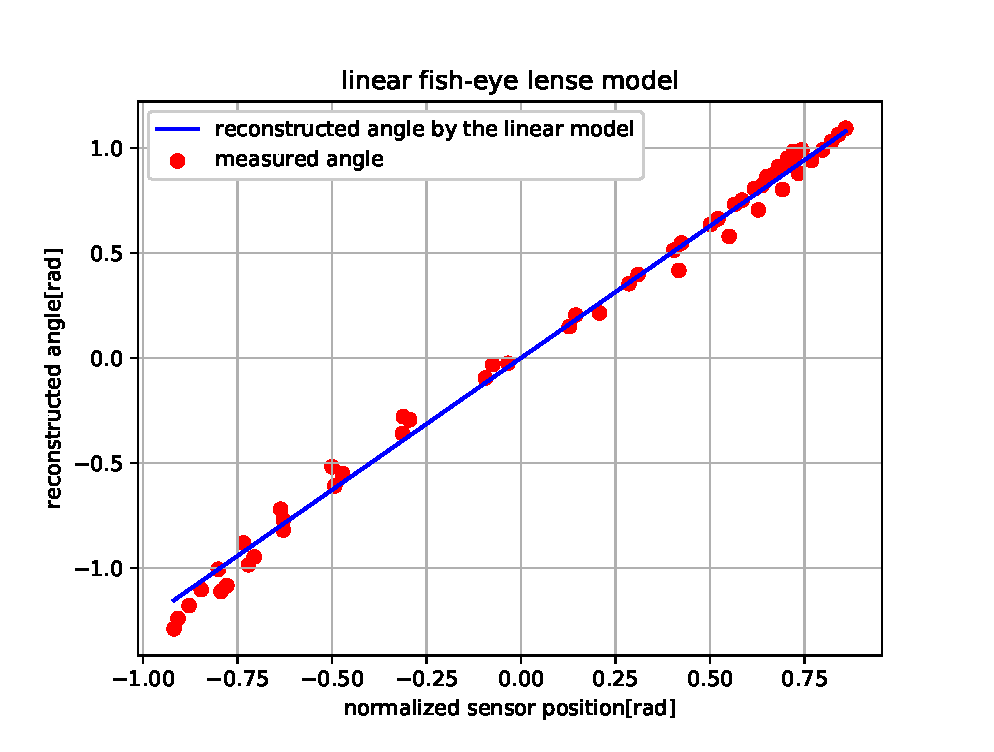
\includegraphics[height=60mm]{fig/linear_model3.eps}
        \caption{The linear model of the lens.}
        \label{fig:linear_model}
    \end{subfigure}
    \qquad
    \begin{subfigure}[Sample1]{0.5\linewidth}    
        \includegraphics[height=60mm]{fig/tan_model2.eps}  
        \caption{The tangent model of the lens.}
        \label{fig:tan_model}
    \end{subfigure} 
    \caption{Approximation of the calibration data by a linear and tangent model of the lens.}
\end{figure}


%\begin{figure}[h!]
%\centering
%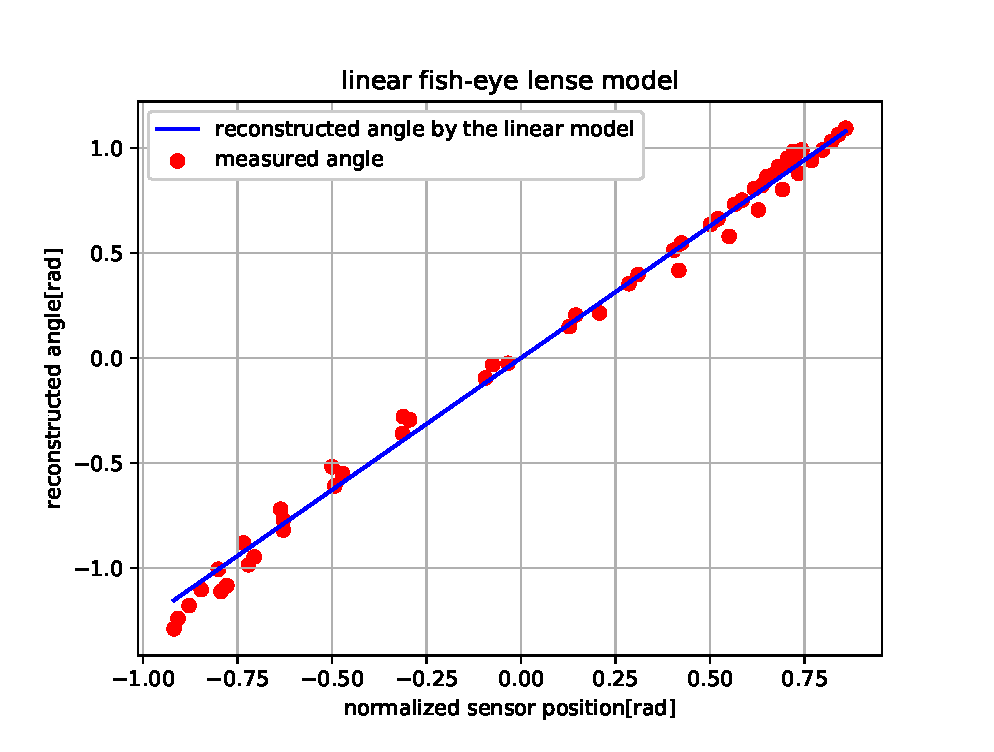
\includegraphics[width=1\linewidth]{fig/linear_model3.eps}
%\caption{The linear model of the lens}
%\label{fig:linear_model}
%\end{figure}

The linear model somehow estimates the real one, but not that well.

\subsubsection{Tangent model}

This is a more complicated model, which is based on the pinhole camera model.

\begin{equation}
\theta^w = f(r^f) = \theta^w \cdot FOV,
\end{equation}

Fitting of the model is shown in the fig.\ref{fig:linear_model}

%\begin{figure}[h!]
%\centering
%\includegraphics[width=1\linewidth]{fig/tan_model2.eps}
%\caption{The tangent model of the lens.}
%\label{fig:tan_model}
%\end{figure}

This model represents the camera optics much better and was chosen to be the final one.

\subsection{The city coordinate system}

There is many ways how to represent real world for representing the car in the city. The most obvious one would be represent the position by longitude, latitude and elevation. This would be correct, but not very practical. Since the distances between same circles of latitude and longitude are different, this would need more complicated transformations and there is a simpler model. 

Since we care only about only one city, we will use a city cartesian coordinate system $(x^c, y^c)$. We can choose any position and rotation of the coordinate center. All we need to know is the relative translations and rotations of each camera $(\Delta x, \Delta y, \Delta\phi)$ to the city coordinate system. For simple transformations we will use homogeneous coordinates, which are in form of $(x, y, 1)^T$. 


A point from a camera coordinate system $(x^w, y^w)$ is transformed to the city coordinate system $(x^c, y^c)$ by a standard 2D rotation and translation matrix as
\[
  \begin{bmatrix}
    x^c \\
    y^c \\
    1
  \end{bmatrix}
   = 
  \begin{bmatrix}
    cos\Delta\phi & -sin\Delta\phi & \Delta x\\
    sin\Delta\phi & cos\Delta\phi & \Delta y\\
    0 & 0 & 1
  \end{bmatrix}   
  \cdot 
  \begin{bmatrix}
    x^w \\
    y^w \\
    1
  \end{bmatrix}
\]







\clearpage
\section{Dataset generation}
\label{sec:classical}

A vehicles detection and tracking without using deep learning has been explored. For several reasons described in this section it has not been used for the final product, but allowed a much faster video annotating, than standard methods and was used to create dataset for training similarity between vehicles described in the section \ref{sec:similarity}

\subsection{Need for a custom dataset}

There are available datasets for image classification and object detection, such as ImageNet \cite{krizhevsky2012imagenet}, COCO \cite{lin2014microsoft}. They also contain images of cars, people, trucks and other classes. However, The section \ref{sec:mask-rcnn} shows, that these datasets can not be used on their own because of the angle, lens type and other factors.

\begin{figure}[h!]
    \begin{subfigure}[Sample1]{0.5\linewidth}
        \includegraphics[height=50mm]{fig/coco0.jpg}
        \caption{Example of COCO photo for object detection.}
        \label{fig:coco0}
    \end{subfigure}
    \qquad
    \begin{subfigure}[Sample1]{0.5\linewidth}    
        \includegraphics[height=50mm]{fig/imagenet3.jpg}  
        \caption{Example of ImageNet photo for image classification.}
        \label{fig:imagenet3}  
    \end{subfigure} 
    \caption{The car class examples in ImageNet \cite{krizhevsky2012imagenet} and COCO \cite{lin2014microsoft}.}
\end{figure}



In our domain vehicles viewed from directly above or and are very distorted. Creating a dataset from our videos is the only way to train an object detection network. 


\subsection{Distributed system}
This section, apart from dataset generation, introduces a computationally fast solution capable of running on CPU inside cameras.

The final system needs to be easily scalable and a particular system architecture has been explored. If the detections and tracking were computed on-board of the cameras, that would help greatly. There would be much less communication needed. Instead of transferring whole video streams, only some meta-data would be sent. That would include: 

\begin{itemize}
\item Time stamps of a frames.
\item Locations of objects and their classes.
\item Some description vector of the detections.
\item Detections clustered to tracks.
\end{itemize}

This system could be greatly distributed sending packets of information among only the cameras that the information is relevant to.

However this has some downfalls, mainly in computational manner. Each camera would have to be equipped either with a capable computational unit. The detections, tracking and similarities would all have to be computed onboard. Since it is not possible to have a GPU in every lamp for many reasons, for example it is a very wet environment, usage of neural networks would not be possible. This section introduces non deep learning approach for detection, tracking and classification, that could run on CPU.



\subsection{Background subtraction detection}
\label{sec:bgs}

Probably the best classical detection methods from static videos, that can be computed in real time on limited hardware, are based on the background subtraction algorithm \cite{piccardi2004background}. The main idea is creating a model of the scene without the objects that we want to detect and then subtracting the current frame and by thresholding determine, where the vehicles are. This simple approach does not work very well and some improvements need to be made. 

For the background subtraction procedure, a model of the background has to be found. For our purposes we need to know, how the road looks like without any vehicles and people. This can't be done by simply waiting for such a case, because the traffic is usually quite high. Instead, we need to figure out the background from multiple frames. 


The algorithm has been implemented in opencv \cite{opencv}. The background is usually created by the mean over several images called running gaussian average \cite{wren1997pfinder}. The idea is to estimate a gaussian to each pixel independently. Each pixel is updated with each new frame as a weighted sum. The background looks like a photo with a long exposition and the lane. In places, where vehicles drive, are colored lines as shown in the figure \ref{fig:cut_mean}. When computed the difference from a video frame to such a background model, as shown in the figure \ref{fig:threshold_mean}, the places, where usually cars drive, can have high values. This can be bad for creating a mask by thresholding, because a higher thresholding constant has to be set.

\begin{figure}
    \begin{subfigure}[Sample1]{0.5\linewidth}
        \includegraphics[height=37mm]{fig/background_mean_crop.png}
        \caption{Mean model.}
        \label{fig:cut_mean}
    \end{subfigure}
    \qquad
    \begin{subfigure}[Sample1]{0.5\linewidth}    
        \includegraphics[height=37mm]{fig/background_med_crop.png}  
        \caption{Median model.}
        \label{fig:cut_med}  
    \end{subfigure} 
    \caption{Background model created by the mean and the median approach.}
\end{figure}

The background model changes with every new frame. In the first iteration, the background $B_0$ is just the first frame $F_0$. The background in next iteration is just the weighted sum of the  current frame and the background model in the previous iteration.

\begin{equation}
B_n = \alpha \cdot F_n + (1 - \alpha) \cdot B_{n-1}
\end{equation}

This algorithm is very fast and can be highly parallelized and computed on graphics cards. The picture having $N$  pixels, the complexity of this standard background subtraction algorithm is  $O(N)$.



\begin{figure}
    \begin{subfigure}[Sample1]{0.5\linewidth}
        \includegraphics[height=37mm]{fig/threshold_mean_crop.png}
        \caption{Mean.}
        \label{fig:threshold_mean}
    \end{subfigure}
    \qquad
    \begin{subfigure}[Sample1]{0.5\linewidth}    
        \includegraphics[height=37mm]{fig/threshold_med_crop.png}
        \caption{Median.}
        \label{fig:threshold_med}    
    \end{subfigure} 
    \caption{The difference between the frame and a background shown in a gray-scale.}
\end{figure}

An improved way of acquiring background model has been used, which greatly improves the quality of current background subtraction methods. A simple change of taking the median instead of the mean at each pixel position gives much better estimation of the background \cite{bgs-med1, bgs-med2}. The algorithm keeps a queue of $K$ images in a memory and with each incoming frame it puts it in the database and for each pixel it computes a median from the queue. This algorithm can be implemented with the complexity $O(N \cdot log(K))$, if we insert each pixel from an incoming frame to a sorted structure. In reality, for small $K$ this would slow the algorithm, because in opencv and numpy there is a great support for working with the whole images. This approach is simply compute the median over all the images from the queue. The complexity is $O(N \cdot K \cdot log(k)).$ The $K$ has been set to 35. The histogram of a particular pixel position over the queue is show in the figure \ref{fig:pixel_hist}.


This turns out to work much better, but still has its limits. If the traffic is very high and vehicles occupy in average more than half of the ground, the background model will fail, but mean approach would fail as well. 

\begin{figure}[h]
\centering
\includegraphics[width=1\linewidth]{fig/pixel_hist.eps}
\caption{The histogram of a particular pixel over 100 images with computed medians.}
\label{fig:pixel_hist}
\end{figure}

Some more complicated models based on unsupervised learning, such as clustering or taking the most frequent bin from histogram for each pixel position could be used, but they would be computationally too complex and would not be practical for realtime video.

The difference between background model and the current frame is very noisy and some filtration has to be made. Before subtraction, the background and the frame has been filtrated with a gaussian filter with the size 3x3 for smoothing. This compensates for the camera vibrations. Then smoothed again with the filter 11x11. This serves as an apriori probability. The idea is, that if there are big differences in the neighboring area, it is a higher probability of the pixel belonging to the car. This also helps to detect gray and black cars, which have similar color to the road. Another advantage is, that this greatly reduces noise and helps to detect vehicles as whole.

This differential image is thresholded and a mask is obtained as shown in the figure \ref{fig:mask_area}. Each blob is presented with a contour and they are thresholded once more by the area. The resulted blobs become detections and a bounding box is created.

\begin{figure}
    \begin{subfigure}[Sample1]{0.5\linewidth}
    	\includegraphics[height=80mm]{fig/frame_cropped.png} 
        \caption{A frame for detection.}
        \label{fig:frame_for_detection}   
    \end{subfigure}
    \qquad
    \begin{subfigure}[Sample1]{0.5\linewidth} 
    	\includegraphics[height=80mm]{fig/mask_area.png}
        \caption{The detections and areas of contours.}   
        \label{fig:mask_area}
    \end{subfigure} 
    \caption{The background subtraction detection algorithm.}
\end{figure}

The background must be continuously adapting to the scene, but the rate of adapting is crucial. If the background is changing too slowly, it will not work very well with changes of lightning from coming clouds, etc. If the background adapts too fast, it will start to contain cars, that stop at the cross section and when the cars leave, this will become a new false detection. From experiments, there is no optimal adapting rate and it depends on the scene, weather and even then these problems will not completely disappear. One small advantage is filtering detections while adapting background.

Background subtraction is a very fast detection algorithm and when having perfect conditions, it is very accurate and The bounding boxes are more precise than most deep learning approaches.

Unfortunately it has many downsides:

\begin{itemize}
\item Moving trees and their shadows create false positives.
\item Overlapping vehicles are detected as only one.
\item It works bad in high traffic, because it can't create a correct background model.
\item It is very sensitive to changes of lightning, such as moving clouds.
\item It is very sensitive to correct setting of hyper-parameters.
\end{itemize}

Most of these points relate to changing background. Especially if the scene is partially cloudy and the lightning changes a lot, the background model needs to adapt quickly. On the other hand, if in the scene is a traffic light, cars spend a lot of time on one spot and could be incorporated to the background model. Not only the car will not be detected, but a false positive will be detected when the car leaves.

For these problems, background subtraction alone can't be used as a good detector, but on perfect scenes  it can be very useful for collecting high quality training data for neural networks detectors, as described in the section \ref{sec:ssd-implementation}.

\subsection{Optical Flow tracking}
\label{sec:optical-flow}
The detections have been described in section \ref{sec:bgs}. Having only the detections for each frame does not give us that much information. We need to connect these detections to a track.

A custom set of algorithms has been implemented in opencv\cite{opencv} for extending the background subtraction algorithm to tracking. Optical flow \cite{optical-flow} is used for a motion estimation in a video. It pairs pixels in two subsequent frames. In other words, it is a discrete 2D vector field, where each vector is a displacement vector showing the movement of points from first frame to second.

The computation of optical flow over the whole image is usually a very expensive procedure. The method used is Lucas-Kanede method \cite{lucas-kanede}. 

This computation is not used on whole image. That would be computationally too expensive and would not be feasible for limited computational resources and realtime system. Instead, each detection is extended for a one optical flow point. In the next frame, this point will move with the object. Each detection is characterized through this point. 

This extends the detector for object tracking and partially solves the problem of two overlapping vehicles. If two vehicles drive close to each other, background subtraction would start to treat them as one object. This improved model will detect this situation and try to keep the bounding boxes on the different vehicles. 

In first experiments, when a new detection appeared, the position of the optical flow point was selected with the Shi-Tomasi \cite{shi-tomasi} algorithm, which is an improved version of the Harris corner and edge detector \cite{harris}. It tries to find some features, that have high gradient and will be easier to track, rather than selecting just the muddle of the bounding box.

In a perfect scenario the algorithm could be used without further improvements. However in real world scenario, false positives, as well as false negatives detections must be dealt with. Furthermore trees and lamps also complicate the situation greatly. When a vehicle drives behind some sort of a pillar, the optical flow point can not be matched with a next frame and stays on the same place in the frame. When the vehicle completely passes, the tracking is lost. A feature had to be added, which is an additional centering of the optical flow point to the middle of the bounding box. with each new frame, the optical flow point moves with the vehicle, but is also moved towards the middle of the bounding box. This solves the issues of the pillar obstacles, but excludes using the Shi-Tomasi and Harris features. 


The tracking algorithm has been described by a set of rules. The main ones are:
\begin{itemize}
	\item If an optical flow point is outside the background subtraction mask, it becomes a 'zombie'.
	\item If a background subtraction detection is without an optical flow point and there is no 'zombie' in the detection, optical flow point is created in the middle of the bounding box. 
	\item If a zombie is not recovered in 10 frames, it disappears. 
	\item If there are more optical flow points in one background subtraction detection, the bounding boxes continue movement with a low pass filter.
	\item The optical flow points are forced to the middle of the bounding box. This solves the problem of the detection being put on the front of the car while coming and due to noise later being outside the bounding box, when the vehicle is viewed from a side. 
\end{itemize}

These improvements work surprisingly well and solve the tracking problem to some extent. If vehicles overlap completely, this approach will fail, but so will most of the other ones. 

\subsection{Classification}
There are many objects detected in a frame and need to be classified. The most important classes are person and a vehicle. If a classification was accurate, simple scenes could be annotated 100\% automatically. That would mean gaining labeled data almost for free and creating huge amounts of datasets for object detection networks.

A simple classifier has been introduced using Haar features \cite{haar} and the SVM classifier. Each Haar feature is a difference of average brightness level in two rectangular areas in the image. 87 distinct haar features were extracted and a vector of real numbers was created representing the image. This vector was the input into a SVM classifier.

The SVM classifier has been trained on 8144 images of cars and 10567 images of people. This dataset was extracted from the fisheye traffic videos provided to us, using the methods described in the section \ref{sec:data-generation}. The test set split ratio was 0.2.

Accuracy on the test set was 0.842. That is quite a good score without using neural networks, but still too far from deploying on the final project or dataset creation and it was not used.

\subsection{Semi-supervised dataset generation} 
\label{sec:data-generation}

\begin{figure}[h!]
\centering
\includegraphics[width=0.5\linewidth]{fig/omni_labeling.png}
\caption{The dialog from the annotation tool.}
\label{fig:labeling}
\end{figure}

Standard annotation approaches for image detection training need the annotator to draw a rectangle and assign it a class for every detection. This is very time consuming and therefore costly. Video is usually around 25 frames per second, so to annotate a minute of video means annotate a 1500 images. This process can be made easier by skipping some frames and moving the bounding boxes around. For the skipped frames linearly approximate the movement of the objects. This can speed up the process, but it still takes a very long time. 


The algorithms introduced in this section can not be used for the final product, mainly because of the problems described in the section \ref{sec:bgs}. However that does not mean, that this can not be used for other purposes. As mentioned before, it works very well on easy scenes. The bounding boxes are precise and this can help the annotator to annotate scenes faster and more precisely, than standard approaches. the annotator is presented a dialog as shown in the figure \ref{fig:labeling}. That includes the whole track, which is annotated by a user through one click. 


Because of the not perfect classifier, classification is done by user. The annotator manually selects the class of the detected track.


\clearpage
\section{Convolutional Neural Networks}

Deep learning is used for artificial intelligence models, which use more non-linear layers of computation. Most common are the Artificial neural networks. They are a computational model inspired by a brain, that can be thought various tasks from image classification \cite{szegedy2016rethinking} to speech processing \cite{graves2013speech}. In this section we will focus on convolutional neural networks for image processing.

\subsection{Inspiration by biology}
Brains are incredibly capable of processing images. Half of a human brain is either directly or indirectly devoted to vision \cite{mit-vision}. Vision can also be very parallelized process, which is how a brain is structured.

The basic computational unit in a brain is a neuron. A neuron in a brain has an input and an output. The input is a dendritic tree, which is connected to outputs(axons) of another neurons. Neurons are only unidirectional and their output is binary. They either fire, if the input is strong enough or they don't. Their connections to other neurons can vary from very weak to a very strong ones and their size can change by learning.

The basic element artificial neural networks is also a neuron. It also has several inputs and one output. The most common neuron can be also called a perceptron\cite{rosenblatt1958perceptron}, which is a well known classifier. The basic function of a neuron can be described as $f(\overrightarrow{\omega} \cdot \overrightarrow{x} + b)$, where $\overrightarrow{x}$ is the input of the neuron, $\overrightarrow{\omega}$ is the output and $f$ is the activation function and $b$ is the bias. The weights and the biases are the only thing, that changes during the training, where the goal is to find such a weights and biases, that the neural networks performs the required task well.

When an architecture is created, the neural network needs to learn how to perform the required task. It figures that out in a training phase from showing the network many input data with labels, for example many pictures and classes of the objects in the images. This is called a supervised learning. After the training phase, the weights are frozen and the network can perform the task, that is was trained to do.

While the structure of the neural network is inspired by the brain, the training is not. The way it is performed is explained more in detail in the section \ref{sec:back-prop}.

\subsection{Layers}
Neurons in artificial neural networks, similarly like in a brain, are organized in layers. These layers are usually connected to each other in a serial way. Neurons in one layer perform the same function. There is more types of layers depending on the neuron's function and the way they are connected. The information describing this defines the neural network architecture.


\subsubsection{Convolutional layer}

\begin{figure}[h!]
    \begin{subfigure}[Sample1]{0.5\linewidth}
    	\includegraphics[height=40mm]{fig/conv1.jpeg} 
        \caption{An example of a convolutional layer.}
        \label{fig:conv_layer}   
    \end{subfigure}
    \qquad
    \begin{subfigure}[Sample1]{0.5\linewidth} 
    	\includegraphics[height=40mm]{fig/conv2.jpeg}
        \caption{Model of a neuron.}   
        \label{fig:neuron}
    \end{subfigure} 
    \caption{Examples of neural networks concepts from \cite{karpathy2016cs231n}.}
\end{figure}

The convolutional layer is a set of neurons placed in a grid of size $m \times n \times k$. Each neuron is connected to a local region in the previous layer. Each neuron performs the function $f(\overrightarrow{\omega} \cdot \overrightarrow{x} + b)$ shown in the figure \ref{fig:neuron}. Thanks to their regular structure and sharing parameters they perform a convolution function, where they look for a different features in the previous layer. The neurons in lower layers can detect edges or lines, while neurons in higher layers can detect eyes or wheels. The neurons can be in a sparser grid relative to the previous layer with gaps called stride, downsampling the previous layer. 

A better insight to this phenomena has been described in \cite{zeiler2014visualizing}.

\subsubsection{Pooling layer}
\begin{figure}[h!]
    \begin{subfigure}[Sample1]{0.5\linewidth}
    	\includegraphics[height=40mm]{fig/pool1.jpeg} 
        \caption{Pooling downsamples the previous layer.}
        \label{fig:conv_layer}
    \end{subfigure}
    \begin{subfigure}[Sample1]{0.5\linewidth} 
    	\includegraphics[height=40mm]{fig/pool2.jpeg}
        \caption{Max pooling operation.}   
        \label{fig:neuron}
    \end{subfigure} 
    \caption{Examples of pooling concepts from \cite{karpathy2016cs231n}.}
\end{figure}

The image has usually big resolution, but the information gained can be described in much smaller information. Because at the lower levels we care about the relative positions of different features, such as lines or colors a lot, with the higher level, where the generalization is bigger, the dimension of the network usually becomes smaller. Pooling neuron takes a set of inputs and returns only one output as the highest input(max pool) or the average of the inputs(average pool). The pooling layer\cite{scherer2010evaluation} is an important part of almost all convolutional neural networks and it can not be trained since it does not have any parameters.

\subsubsection{Fully connected layer}
In the fully connected layer, each of the neurons is connected to every neuron in the previous layer. Since the layers can have many neurons, this is a very expensive operation and is usually performed at the last layers of the network, where the layers are smaller. They are used as the final classifier, each neuron representing one class.

\subsubsection{Overfitting and dropout layer}
The neural network has many parameters and high Vapnik-Chervonenkis dimension \cite{blumer1989learnability}, therefore it is more prone to overfitting. The network should from the training set of examples figure out some basic understanding of the problem and use this knowledge to process a sample, that it has never seen before. Overfitting means, that the network performs well on the training set by learning it by heart, but fails on the test set. This is a general phenomena in machine learning. Usually the way is to select a simpler classifier, that can still handle the problem or increase the training data. Neural networks have come up with a solution called dropout, which does not solve the problem completely, but greatly helps. 

A neuron in a dropout layer has only one input and during training randomly copies its value to the output or returns a zero. This forces the network to build more robust connections. This layer is active only during training. 


\subsection{Backpropagation}
\label{sec:back-prop}
As mentioned before, the learning of artificial neural networks is very different from learning of a real brain. With each input example, the network performs a forward pass. The informations flows from one layer to next layer and the operations are performed until the information reaches the output layer. Information is compared with the ground truth embedding and a backpropagation is performed, that changes the parameters of the network in a way, that next time the output is closer to the required embedding. The difference is called loss and there are different ways to compute it.

The simplest square loss is computed as 

\begin{equation}
 L(\overrightarrow{y}) = - \sum_{i=1}^N(y_i -  \hat{y_i})^2.
\end{equation} 

After each forward pass, backpropagation finds a gradient for each weight and bias $\omega$, that minimizes the loss and changes it in the direction. 

\begin{equation}
\omega_{t + 1} = \omega_{t} + \frac{\partial L(\overrightarrow{y_t})}{\partial \omega}
\end{equation}

This general process is called a gradient descent. Backpropagation is an efficient way how to  compute these partial derivatives from back to front of the network based on the chain rule.

\subsection{Transfered learning}

Since filters in lower layers detect just very simple features, in comparison to higher layers, they are not too domain specific. If a network was trained on images of animals and was to be retrained to detect vehicles, the higher level filters for detecting eyes or legs could not be used. In contrast, the low level features detecting edges or lines could stay unchanged. This is the high level idea of transfered learning. Training the network on a different domain and retraining it for a different one. 

This has many advantages. Training of the lower layers is more difficult because of the vanishing gradient problem. Training of these layers also requires a huge amount of data and computational time. There are many different pretrained networks available online. Using such a network and only fine tuning it to a specific task requires also less training data. However, this is possible only for the exactly same architectures of the networks.

\subsection{Frameworks}
Artificial neural networks require sometimes billions of very simple operations. Although they have been known for many years\cite{widrow199030}, only recently they have had a great success. That is due increased computational power, parallelizing the computations on GPU, which perform these operations much faster than CPU and access to a big amount of data. 

There are also some frameworks, that offer very fast computations on GPU such as Google's TensorFlow \cite{abadi2016tensorflow}, Theano \cite{bergstra2011theano} or CNTK\cite{seide2016cntk} by Microsoft, from which the TensorFlow is the most common and the reidentification part of the thesis described in the section \ref{sec:similarity} has been implemented in this framework. 

There are also some libraries such as Keras \cite{chollet2015keras} and Caffe \cite{jia2014caffe} that make implementing deep learning in C++ or python much easier. The SSD object detection network described in the section \ref{sec:ssd-implementation} has been implemented in Keras.


\clearpage
\section{Classification, Detection and Reidentification networks}
\subsection{Neural networks for classification}
\label{sec:neural_networks_classification}
The Neural networks have been the state of the art for the image classification. The driving force has been the ILSVRC \cite{krizhevsky2012imagenet} competition. Classification neural networks are also used as the backbone for detection networks.



\subsubsection{VGG}
\label{sec:vgg}

\begin{figure}[h!]
\centering
\includegraphics[width=1\linewidth]{fig/vgg.png}
\caption{The different VGG architectures. The ReLU function is not shown for simplicity. \cite{simonyan2014very}}
\label{fig:vgg}
\end{figure}

The VGG\cite{simonyan2014very} architecture from Oxford is one of the simplest ones, but is very accurate. It is often used as a base network in object detection networks such as YOLO\cite{redmon2016you}, ARTOS\cite{barz2017fast}, SSD \cite{liu2016ssd} or Faster R-CNN \cite{faster-rcnn}. In this thesis, the VGG network has been used as the SSD backbone and has been adjusted for this specific domain in the section \ref{sec:ssd-implementation}. 

The VGG is an image classification network. It takes an input image and produces a probabilities for each predefined class. It has been inspired by \cite{ciresan2011flexible} and \cite{krizhevsky2012imagenet}.

The input resolution of the network is fixed to 224 $\times$ 224. The idea of the network is to use a very small filters 3 $\times$ 3  (which is the smallest size to capture the notion of left/right, up/down, center)\cite{simonyan2014very}. Two of these filters stacked on top of each other create a receptive field of 5 $\times$ 5 and three have the receptive field of 7 $\times$ 7. With sharing parameters, the three layers has almost half the parameters, than the layer with 7 $\times$ 7 filters. This is different from \cite{krizhevsky2012imagenet} with 11 $\times$ 11 filter in the first layer and \cite{zeiler2014visualizing} with 7 $\times$ 7.

To bring more non-linearity, the VGG16 uses a filters with 1 $\times$ 1 filters. This has been used also in \cite{lecun1989backpropagation} as a network in a network.

Thanks to padding and the stride 1 of convolutional layers, the layers are down-sampled only by 2 $\times$ 2 max-pool layers with stride 2. The number of channels increases for better processing of higher level features. 

Different VGG architectures have been evaluated designed in \cite{simonyan2014very} and shown in the figure \ref{fig:vgg}. 



\subsection{SSD network for detection}
\label{sec:ssd}

The state of the art in detection is at the time the Single Shot MultiBox detector \cite{liu2016ssd}. This network provides accurate realtime object detections (74.3\% mAP at 59fps on VOC2007 on GPU). They achieve much faster speed, compared to previous Faster R-CNN (7 fps on GPU) thanks to eliminating the bounding box proposals. Since the SSD architecture is much simpler and compact, than R-CNN architectures, the training is performed end to end on a single model, instead of training multiple networks for region proposal, classification and bounding box regression.

\subsubsection{Architecture}

\begin{figure}[h!]
\centering
\includegraphics[width=1\linewidth]{fig/SSDvsYOLO.png}
\caption{Comparison of the SSD\cite{liu2016ssd}(300x300) and YOLO\cite{redmon2016you}(448x448) architectures.}
\label{fig:ssd_vs_yolo}
\end{figure}

The SSD network uses one feed forward flow to produce a fixed number of bounding boxes and their probability for each class. The early layers are sometimes called a base network or a backbone. They are a classical architecture for image classification. 

Some additional layers have been added on top of the base network show in fig. \ref{fig:ssd_vs_yolo}. Multi-scale feature maps for detection are convolutional layers that progressively decrease their size and allow cheap detections of multiple scales. Convolutional predictors for detection can from feature maps of size $m \times n$ with $p$ channels can predict scores for categories or the offsets for each $3 \times 3$ element  using small kernels of $3 \times 3 \times p$. With decreasing feature maps, the predictions relate to different object scales. The bounding boxes offsets are measured relative to the each feature map location. 

\subsubsection{Default boxes and aspect ratios}
Each feature map cell, from the feature maps at the end of the network, is associated with a set bounding boxes. They differ in shape and scale as shown in the figure \ref{fig:ssd8}. Since the feature maps are computed from convolutions and max pool layers, the bounding boxes regularly tile the input image as shown in the figure \ref{fig:ssd8} with fixed positions.

A prediction of a probability of each class and predicted offset of the the bounding box is computed. The offsets are given relative to the associated fixed position of the bounding box as shown in the figure \ref{fig:ssd4}. For predicting $k$ shapes and $c$ classes with 4 numbers representing the translations $\Delta(cx, cy, w, h)$, we need $k(c+4)$ filters for each feature map cell and for one $m \times n$ feature map layer we need $mnk(c+4)$ filters. The default boxes are similar to anchor boxes in Faster R-CNN with the difference, that SSD uses multiple feature maps for different object scales. 


\begin{figure}
    \begin{subfigure}[Sample1]{0.3\linewidth}
    	\includegraphics[height=35mm, width=35mm]{fig/ssd_dog_cat.png} 
        \caption{SSD prediction.}
        \label{fig:ssd_detection}   
    \end{subfigure}
    \quad
    \begin{subfigure}[Sample1]{0.3\linewidth} 
    	\includegraphics[height=35mm, width=35mm]{fig/ssd_feature_map.png}
        \caption{8 $\times$ 8 feature map.}   
        \label{fig:ssd4}
    \end{subfigure} 
    \quad
    \begin{subfigure}[Sample1]{0.3\linewidth} 
    	\includegraphics[height=35mm, width=35mm]{fig/ssd_4_feature_map.png}
        \caption{The predicted offsets.}   
        \label{fig:ssd8}
    \end{subfigure} 
    \caption{The background subtraction detection algorithm.}
\end{figure}

\subsection{Loss}
*** todo ***

\subsubsection{Training}
With each training image, the ground truth boxes need to be assigned to a default bounding box. The ground truth box is matched to all default boxes, which have the Jaccard overlap higher than 0.5. This is more robust, than picking only the one box with the highest overlap as in MultiBox \cite{erhan2014scalable}. After that, the training is performed end to end by a standard backpropagation. 

The training phase also includes a positive and a hard negative mining. Not all predicted boxes participate on training. Most of the predicted boxes are usually negatives. The backpropagation is on all the boxes matched with ground truth box as well as the negatives with lowest score for background. This is called hard negative mining and it speeds up the convergence. The negatives are picked with the ratio 3:1 to the positives.

\subsection{Non maxima suppression}

\begin{figure}[h!]
	\begin{subfigure}[Sample1]{0.5\linewidth}
    	\includegraphics[height=50mm, width=50mm]{fig/nms1.png} 
        \caption{Predictions before applying nms.}
        \label{fig:nms1}   
    \end{subfigure}
    \quad
    \begin{subfigure}[Sample1]{0.5\linewidth} 
    	\includegraphics[height=50mm, width=50mm]{fig/nms2.png}
        \caption{Predictions after applying nms.}   
        \label{fig:nms2}
    \end{subfigure} 
\caption{Non maxima suppression\cite{diez2011non} keeps a single prediction.}
\label{fig:nms}
\end{figure}

Detectors usually create many predictions around an object as shown in the figure \ref{fig:nms1}. The goal of non maxima suppression is to keep only a single bounding box. 

Each prediction has a confidence. Non maxima suppression sorts all predictions by their confidence. It takes a prediction with the higher confidence and finds all predictions with a Jaccard overlap\cite{tan2005introduction} higher than some constant, removes them and moves to next prediction. This is a naive approach and use of k-d trees can speed up the process.

The constant is the only parameter of the algorithm and setting it is a very important thing. If set too high, objects will have multiple detections. If set too small, objects, that are close together, will be detected as one. The rule of thumb is to set the constant between 0.3 and 0.5.


\subsection{Facenet for reidentification}
\label{sec:facenet}
Google Facenet \cite{schroff2015facenet} is a deep neural network for computing similarities between faces, but can be retrained for computing similarities between objects from any domain, such as vehicles. This network  receives an input image in rgb with the size of $220 \times 220$ and returns a embedding vector with the length of 128. The euclidean distance between samples directly corresponds to the similarity of objects. Faces of the same person are mapped to the similar place in the euclidean space. Once we have this metrics, recognition becomes a K-NN and verification is a simple thresholding of the distance. The goal is, that the embeddings will be invariant to pose, illumination and other factors. For computing the similarity of an image with more images representing the same identity, a mean of the distances is taken.

\subsubsection{Architecture}
\begin{figure}
    \begin{subfigure}[Sample1]{0.5\linewidth}
    	\includegraphics[width=0.95\linewidth]{fig/facenet.png} 
        \caption{The model structure.}
        \label{fig:facenet_structure}
    \end{subfigure}
    \quad
    \begin{subfigure}[Sample1]{0.5\linewidth} 
    	\includegraphics[width=0.95\linewidth]{fig/triplet_loss.png}
        \caption{The learning objective.}   
        \label{fig:triplet_loss}
    \end{subfigure}
    \caption{The Facenet \cite{schroff2015facenet}.}
\end{figure}

The facenet architecture is mostly an image classification network for 128 categories and a normalization layer. Google has tried various architectures, such as Zeiler\&Fergus \cite{zeiler2014visualizing} (with the input resolution 220 $\times$ 220), Google Inception \cite{szegedy2016rethinking} (224 $\times$ 224, 160 $\times$ 160, 96 $\times$ 96) and mini Inception (165 $\times$ 165) and tiny Inception(140 $\times$ 140). 


The \cite{szegedy2016rethinking} shows, that the embedding space dimensionality of 128 is enough for recognizing faces.

\subsubsection{Training}
The training and evaluation data are sets of images of different people. The goal of the network is to project images of the same person close to each other and different people far from each other as shown in the figure \ref{fig:triplet_loss}. This is a different problem, than classification, where a finite number of categories is previously known. There have been been attempts \cite{wst2008deeply, taigman2014deepface} for training network for classification and then removing the last classification layers, but with less success.

The introduced approach is different from an image classification training and is called triplet loss. With each training step, three examples are selected. Two of the same class and one from a different one. One of the positives is called anchor, the one from the same class is called a positive and the third one a negative sample. The goal is to change the network parameters in a way, that the positive embedding is moved closer to the anchor and the negative further from the anchor.

The triplet loss is represented as $f(x) \in R^d$, where $x$ is the input image that is transformed into an Euclidean $d$-dimensional space. The last normalization layer normalizes the embedding to a hypersphere of the size 1, meaning $\|f(x)\|_2 = 1$ 

To ensure, that the model is consistent, meaning, that there exists a threshold, that will correctly classify every pair of the images, we need to ensure, that for $\alpha = 0$

\begin{equation}
\begin{aligned}
&\|f(x_i^a) - f(x_i^p)\|^2_2 + \alpha < \|f(x_i^a) - f(x_i^n)\|^2_2 \\
&\forall (f(x_i^a), f(x_i^p), f(x_i^n)) \in T
\end{aligned}
\end{equation}

The $\alpha$ is a constant, that can enforce a margin. $T$ is a set of all possible combinations of images in the training set.

The loss, that is being used for training according to \cite{szegedy2016rethinking} is 

\begin{equation}
\sum_i^N [\|f(x_i^a) - f(x_i^p)\|^2_2 - \|f(x_i^a) - f(x_i^n)\|^2_2 + \alpha]_+.
\end{equation}

After couple of steps of training, most of the images will be classified correctly and the constraint will be met. For fast convergence, it is crucial to select those triplets, that violate the condition. This is called hard positive and hard negative mining.

There have been recently some improvements of triplet loss in form of quadruplet loss \cite{chen2017beyond}, that enforces grater margins among classes.

\subsection{Multi camera tracking}
\label{sec:multi-camera-tracking}
After solving the task of detection, single camera tracking and similarity metrics, The task needs to be extended to the whole city. It is important to note, that a the city with built cameras in lamps does not exist at the time of writing the thesis, therefore these ideas can not be tested on the whole city. Only a theoretical approach has been explored. It is also important to keep in mind the task of tracking one vehicle in a city, therefore not tracking all vehicles at once, which can 


\clearpage
\section{Implementation}

The deep learning runs in TensorFlow \cite{abadi2016tensorflow} framework. Keras \cite{chollet2015keras} was used for implementation and development of neural networks, opencv \cite{opencv} for video and image operations and numpy \cite{walt2011numpy} for fast vector operations. The whole project was written in python.


\subsection{Mask R-CNN segmentation}
\label{sec:mask-rcnn}

\begin{figure}[h!]
    \begin{subfigure}[Sample1]{0.5\linewidth}
    	\includegraphics[width=0.95\linewidth]{fig/Mask-RCNN-road.png} 
        \caption{Mask R-CNN on a standard street camera.}
        \label{fig:mask-street-cam}
    \end{subfigure}
    \quad
    \begin{subfigure}[Sample1]{0.5\linewidth} 
    	\includegraphics[width=0.95\linewidth]{fig/Mask-RCNN-omni.png}
        \caption{Mask R-CNN on a fisheye has problems recognizing vehicles from the top.}   
        \label{fig:mask-omni-cam}
    \end{subfigure}
    \caption{Examples of Mask R-CNN network \cite{he2017mask}.}
    \label{fig:facenet}
\end{figure}

First, couple of approaches were explored, but not to a great detail. One of them is Mask R-CNN\cite{he2017mask}. This network builds on detections and provides segmentation. This gives more information, since we know exactly what parts of objects belong to which entity, making the tracking simpler. As shown in the figure \ref{fig:mask-street-cam}, Mask R-CNN can very well detect standard traffic scenes, however, in the figure \ref{fig:mask-omni-cam}  one can see, that it has problems detecting vehicles from the top. This is due to a very small number of vehicles viewed right from the top in the Microsoft COCO dataset \ref{lin2014microsoft}. 

Since there are no datasets for training and evaluating segmentation from the top-places fisheye street cameras the performance has not been measured. Transfered learning could be applied, but creating such a segmentation dataset is very expensive to create. Combining this fact with the 5 fps of this network, it is not feasible for realtime application and this approach has not been explored further. 

However, it is a valuable insight and when segmentation becomes faster, this is definitely an approach worth looking into in the future work.

\subsection{SSD detector}
\label{sec:ssd-implementation}
The most important part of the thesis is the vehicle detection. This is a very hard problem given the conditions. First of all, since the camera is fisheye, it is not possible to simply use a off the shelf network trained for example on ImageNet or on PASCAL VOC and use it right away. 

For the detector has been chosen the SSD network \cite{liu2016ssd} described in the section \ref{sec:ssd}. It is the state of the art realtime detector outperforming the R-CNN\cite{faster-rcnn} and YOLO\cite{redmon2016you} in speed and accuracy as described in the section \ref{sec:object_detection}. 

the SSD uses VGG-16 for the base network, which has been described in the section \ref{sec:vgg}. VGG networks are popular among detection networks for their performance and simplicity. 

The SSD introduces two versions differing in the input resolution: SSD300 and SSD512 with the resolutions $300 \times 300$ and $512 \times 512$ respectively. Because the cameras are positioned high and because of the fisheye view, objects, especially bicycles and motorcycles, can appear very small. It is sometimes problem for humans to detect them on $1024 \times 1024$ image, therefore the version with higher resolution has been chosen. 

A working network implemented in keras\cite{ssd_keras} has been used as a starting point, but some modifications have been made. 

\subsubsection{Temporal difference}

\begin{figure}
    \begin{subfigure}[Sample1]{0.5\linewidth}
    	\includegraphics[width=0.95\linewidth]{fig/stream_frame.png} 
        \caption{A frame from the street camera.}
        \label{fig:td_frame}
    \end{subfigure}
    \quad
    \begin{subfigure}[Sample1]{0.5\linewidth} 
    	\includegraphics[width=0.95\linewidth]{fig/stream_black.png}
        \caption{Temporal difference highlights moving objects.}   
        \label{fig:td_black}
    \end{subfigure}
    \caption{Temporal difference helps to detect moving objects.}
    \label{fig:td}
\end{figure}

As described in the section \ref{sec:object_detection}, the standard pipeline for video detection is detecting each frame independently. This looses much information, that can be gained from the video. Cameras used in this thesis are static and the vehicles, that are to be detected are mostly moving. A cheap segmentation of the scene is a temporal difference. 

A difference between two subsequent frames is shown in the figure \ref{fig:td_black}. It is computed as:

\begin{equation}
D(F^{T}_{i, j}) = max(255, \sum_{c = 1}^3 |F^t_{i, j, c} - F^{t-1}_{i, j, c}|)
\end{equation}

where $F_{i, j}^t$ is a value of a frame at the time $t$, $i$-th row and $j$-th column. The image is represented in 8-bit unsigned int, therefore to prevent overflow, the value is saturated on 255. The difference between frames can be computed very fast in python using numpy\cite{walt2011numpy} and opencv\cite{opencv} libraries. 

There are more ways, how to use this information in the network. One could feed just this layer and probably achieve good detections, but would have problems with object classification by loosing the rgb information. The introduced approach keeps both the information by feeding both to the network.

The SSD network has been extended for an extra input channel in addition to rgb, that is the temporal difference. The data have size $H \times W \times 4$ instead of $H \times W \times 3$ for standard images. This version of the network has been temporarily called RGBD network. The D stands for the difference and should not be confused with commonly used distance.

In some cases, we don't want to detect parked cars. This is in a case of a road with lot of parked cars and where are no traffic lights. In this case, the tracking will perform better with less bounding boxes and no occlusions with the parked cars. This can be easily done by computing the average value in the difference channel and thresholding it.


\subsubsection{Architecture}
The architecture is similar to the original SSD512 architecture, but some changes have been made. 

The input layer has been extended for the differential channel as described before. 

According to some literature \cite{cao2018feature}, SSD might have problem with detecting small objects. Therefore one more feature layers has been added with a small scaling factor 0.05, compared to the original 0.1. This additional feature layer is able to detect roughly twice as smaller objects as the original network, such as pedestrians, bicycles or motorcycles.

\subsubsection{Dataset}
A scene annotating has been introduced in the section \ref{sec:data-generation}. However this approach could not be used for SSD training and was used only for similarity training described in the section \ref{sec:similarity}. Even though it produces no false positives, sometime it produces false negatives due to the inability of correctly segmenting overlapping objects. It only detects such a situation and does not label anything.

Despite over-all good scene annotation, the SSD's hard negative mining strategy selects the bounding, that the network predicted most likely as a presence of an object and were not labeled and tweaks the weights in such a way, that next time it is predicted as a background. In other words, if a vehicle is not labeled in the image, the network might detect it, but will be corrected, that it is a background. This would lead to a bad learning, overfitting and might not even converge.

A standard online annotation tool has been provided by the goodvision company, that allows annotators to draw bounding boxes and attach classes to images. Several annotators have annotated 1764 images.

The Brazilian party provided 15 videos from different scenes, each about 1 hour long. Each video has been shot from a slope on a car, as shown in the figure \ref{fig:calibration}. Only two cameras in lamps were working and recording video in the time of writing this thesis, since the whole project is still in development. 

The rgb images and the temporal difference have been extracted from the total of 17 scenes a second apart and the images without traffic have been deleted. There is need for many scenes for the diversity of the roads, surroundings and lightning conditions. 

A detector can easily overfit on a scene by learning its background, therefore the test data have been chosen to be one scene, where the detector did not learn.

The dataset contains 1654 training and 110 testing images. Because of the sparsity of the data and not many hyperparameters, the validation set is equal to the test set.

There are 7 classes in the data: 
[person, bicycle, car, bus, motorbike, truck, animal]

The classes person and animal are not important for this project, but might be used for adding new features in the future.
\subsubsection{Data augmentation}
For extending the dataset, many different methods of editing the images are being used. They usually contain horizontal flip, selecting patches or editing brightness. 

The nature of the 360 degree camera enables us to rotate the image in an arbitrary angle, not only a horizontal flip, such as on standard datasets. 

On a standard frame, not all vehicles are moving. Some are parked and some stay at a traffic or on a red light. It is important to detect these also, therefore 4th layer is set to zero with the probability of 0.1 to provide more data for the rgb part of the network.

All the data augmentation techniques used during training are:

\begin{itemize}
\item Random rotation of the image.
\item Random brightness change.
\item Random image translation.
\item Random scaling of the image.
\item Random setting of the 4th layer to zero.
\end{itemize}

\subsubsection{Training}

It is not possible to use pretrained model on ImageNet\cite{deng2009imagenet} or COCO \cite{lin2014microsoft}, because of the changed architecture of the network. A pretrained weights could not be used for transfered learning. An attempt has been made to pretrain the model on Youtube-boundingboxes dataset\cite{real2017youtube}, but only static videos would have to be selected because of the differential input channel and the scenes are too different from the fisheye traffic camera.

The images were shuffled before each epoch. The minimum overlap between anchor and a label has been set to 0.5, the maximum overlap between anchor and background label has been set to 0.2 and the threshold for moving labels from the ground truth during training was set to 0.2. The training was performed on the NVIDIA GeForce GTX 1080 for 4 days.

A custom tensorboard callback and mAP computation had to be implemented for observing the training progress and evaluating the model. Another features were added, such as tracking the  detection ratio or computing the best threshold from the mAP curve. 

The Adam optimizer \cite{kingma2014adam} has been used with parameters: The learning rate $10^{-3}$, $\beta_1 = 0.9, \beta_2 = 0.999, \epsilon=10^{-8}, decay = 0.0005$. These parameters have been selected by \cite{ssd_keras} and were not changed. The training process is shown in the figure \ref{fig:ssd_training}


\begin{figure}[H]
    \begin{subfigure}[Sample1]{1\linewidth} 
    	\includegraphics[width=0.95\linewidth]{fig/ssd_rgbd/mAP.png}
        \caption{The mean average precision on validation set.}   
        \label{fig:ssd_mAP}
    \end{subfigure}
    \begin{subfigure}[Sample1]{1\linewidth} 
    	\includegraphics[width=0.95\linewidth]{fig/ssd_rgbd/loss.png}
        \caption{The loss on the training set.}   
        \label{fig:ssd_loss}
    \end{subfigure}    
	\begin{subfigure}[Sample1]{1\linewidth} 
    	\includegraphics[width=0.95\linewidth]{fig/ssd_rgbd/val_loss.png}
        \caption{The loss on the validation set.}   
        \label{fig:ssd_val_loss}
    \end{subfigure}    
    \caption{The process of training the 4 channel input SSD network. The training was performed on the NVIDIA GeForce GTX 1080 for 4 days.}
    \label{fig:ssd_training}
\end{figure}

The training converged after about 3000 training steps. The final training loss was 0.3035 ant validation loss 0.2201. The mAP on the test set was 91,6 \%.



\subsection{Single camera tracking}

Single camera tracking is the only thing, that has not been implemented by the author of the thesis. The company goodvision provided their own state of the art tracker. It is similar to the tracker explained in the section \ref{sec:optical-flow}, but more advanced.

It requires the video and a sequence of detections and connects these detections to tracks, which are sequences of these detections. This allows non supervised clustering of track in the scene without needing to mark the initial object. 

The tracker works in three steps called seeding, displacement and matching. 

\subsubsection{Seeding}
When a new detection appears, a set of features is initialized. These are as set of points inside the bounding box that have been selected by the Shi-Tomasi \cite{shi-tomasi} feature detector. The Shi-Tomasi chooses features by finding a local maxima in differentiating the image in both axis and choosing the smaller of the two. It usually finds corners or another distinguishing features, that are easier to track by optical flow. 

Because the detection is a bounding box, the features are initialized not only on the tracked vehicle, but also on the background. This is undesirable, since we want to track only the moving object. This could be solved with replacing object detection with segmentation, but would increase the computational time of the detector and make creating datasets harder.

\subsubsection{Displacement}
After features have been initialized, displacement of each feature is computed with the incoming frame. The movement is estimated by optical flow using Lukas Kanede \ref{lucas-kanede} method. Optical flow is computed only for the sparse local features and not for whole frame, making it faster. Those features, that have been initialized on moving vehicle move with it and those on the background stay on the same place. 

\subsubsection{Matching}
Each feature remembers, which object it originally belonged. After the features have been moved in the displacement step, they are matched to the new detection. The features outside detections(those previously seeded on the background) are removed. The detections with features, that belonged to the same previous detection, take its identity and are matched together. This way a track is created.

\subsection{Similarity}
\label{sec:similarity}

\begin{figure}
    \begin{subfigure}[Sample1]{0.5\linewidth}
    	\includegraphics[width=0.95\linewidth]{fig/facenet_eval_table.png} 
        \caption{Mean VAL at $10^{-3}$ FAR.}
        \label{fig:facenet_table}
    \end{subfigure}
    \quad
    \begin{subfigure}[Sample1]{0.5\linewidth} 
    	\includegraphics[width=0.95\linewidth]{fig/facenet_eval.png}
        \caption{Comparison of different DNN architectures.}   
        \label{fig:triplet_loss}
    \end{subfigure}
    \caption{Comparison of various facenet\cite{szegedy2016rethinking} base networks evaluated on Labeled faces in the wild\cite{huang2007labeled} and YouTube faces\cite{wolf2011face} datasets.}
    \label{fig:facenet}
\end{figure}

The neural network Facenet \cite{schroff2015facenet} was chosen as the metrics of similarity among vehicles. As described in the section \ref{sec:facenet}, it is designed to compute similarity between faces and is taught to be invariant to various poses and illumination conditions. The network can be retrained for a different domain apart from faces, in our case vehicles. Given an image of a car, the network will produce an embedding in an 128-d Euclidean space in such a way, that the same objects should be close to each other. Google has tried many architectures, that are compared in the figure \ref{fig:facenet}. The Inception network NN3 with the input resolution of 160 $\times$ 160 is a good trade-off between the speed and accuracy. Furthermore increasing input resolution is not practical for our task, since the resolution of the cameras is only full HD and the vehicles inhabit only  very small area in the frame.

As a starting point, TensorFlow implementation of the network \cite{facenet} has been used. The network stayed unchanged, but the data handling, tensorboard callbacks and evaluation had to be implemented.

\subsubsection{Dataset}
\begin{figure}[h!]
\centering
\includegraphics[width=1\linewidth]{fig/facenet/labeling.png}
\caption{An example of a one object in a training set.}
\label{fig:facenet-labeling}
\end{figure}

The dataset needed for this task is in a form of a set of images of an object for many objects. That means, that we need set of images of the same vehicle for many vehicles. Use of other datasets, such as \ref{standford} is not possible, because their images look too different, from those in the fisheye street camera.

The main idea in creating a custom dataset was, that if we have a track - a set of bounding boxes of the same car on one scene, we can use these detections as a set of images of the same vehicle. That is exactly what the background subtraction and optical flow does. This dataset has been created by a semi-supervised annotation tool based on background subtraction and optical flow described in the section \ref{sec:data-generation}.

Different scenes and different weather conditions have been used for better diversity. The created dataset contained over 9 000 images.

\subsubsection{Problems with the dataset}
When the facenet network was trained on this dataset, it did not work at all. There are couple of big problems that have to do with the way Facenet learns. In each training step it takes two images, that belong to different classes, but have been classified as too similar. If each class contained a different car, this would make no problem. However, vehicles, especially in south America, are very similar. If there is a model of the same car in the database more times, the facenet will be taught, that it is a different car and it needs to change. Especially if the car is in the same scene, it looks almost identical and not even human can tell them apart. 

Another problem is, that if the same model of the car appears on a different scene, there is no match with the original car. The network treats these cars as different. This is the opposite of what we want to achieve.

The final problem considers low diversity among one track. The road is usually of the same color and the lightning conditions barely change. The network can then overfit on these features and will not generalize.

\subsubsection{Improving the dataset}
These problems had to be taken into account when creating a new version of the dataset. It would be very hard for the annotator to remember, which types of vehicles have passed and which did not. Instead, the original dataset had to be clustered. That means putting same vehicles from a different scenes into one class. This is a very time demanding process, but the results are worth it.

\subsubsection{Training}
\begin{figure}[h!]
\centering
\includegraphics[width=1\linewidth]{fig/facenet/acc.png}
\caption{Accuracy during the facenet training.}
\label{fig:facenet_training}
\end{figure}

To extend the dataset, some augmentation techniques have been used, such as rotation of the vehicles by 90\textdegree. Transfered learning has been used and the network pretrained by Google on faces was fine tuned on vehicles. The training took 12 hours (150 000 steps) on the NVIDIA GeForce GTX 1080. The training set contained 8800 images and the validation set 884 images from the clustered dataset. These were models of a vehicles, that the network has not seen before. The accuracy has been computed by changing the task to a classification task described in the section \ref{sec:similarity-eval}

\begin{figure}[H]
    \begin{subfigure}[Sample1]{0.5\linewidth} 
    	\includegraphics[width=0.95\linewidth]{fig/facenet/tpr.png}
        \caption{True positive rate.}   
        \label{fig:facenet}
    \end{subfigure}
    \begin{subfigure}[Sample1]{0.5\linewidth} 
    	\includegraphics[width=0.95\linewidth]{fig/facenet/tnr.png}
        \caption{True negative rate.}   
        \label{fig:facenet}
    \end{subfigure}    
	\begin{subfigure}[Sample1]{0.5\linewidth} 
    	\includegraphics[width=0.95\linewidth]{fig/facenet/fpr.png}
        \caption{False positive rate.}   
        \label{fig:facenet}
    \end{subfigure}
    \begin{subfigure}[Sample1]{0.5\linewidth} 
    	\includegraphics[width=0.95\linewidth]{fig/facenet/fnr.png}
        \caption{False negative rate.}   
        \label{fig:facenet}
    \end{subfigure}       
    \caption{Additional information about the Facenet training. The training was performed on the NVIDIA GeForce GTX 1080 for 12 hours.}
    \label{fig:facenet_training_additional}
\end{figure}

The final results are shown in the table \ref{tab:facenet}.

\subsubsection{T-SNE visualization}
\begin{figure}[h!]
\centering
\includegraphics[width=0.5\linewidth]{fig/tsne0.png}
\caption{Visualization of facenet embeddings using the T-SNE dimensionality reduction.}
\label{fig:facenet_training}
\end{figure}

The facenet transforms the images into a 128 dimensional Euclidean space. It is very hard to understand problems, such as variance of rotation, lightning and so on. Simple distances between images are not enough to understand better of the embeddings. 

Some dimension reduction techniques can be used for the embedding visualization. The most common techniques are PCA\cite{wold1987principal} and T-SNE\cite{maaten2008visualizing}. PCA is better to understand the overall relations, while T-SNE can better visualize the local relations. T-SNE has been chosen and a small batch of car images has been selected. The T-SNE has been computed in python using sklearn\cite{pedregosa2011scikit} package.

The T-SNE algorithm The results are shown in the figure \ref{fig:facenet_training}.

It can be seen, that it can distinguish different colors of cars. However being presented two very similar white vehicles, it has some problems distinguishing them. Also we can see, that the network is not fully rotation invariant, even though it has been trained to be. But we need to keep in mind, that a lot of information has been lost with the dimensionality reduction, therefore the preview is not very reliable.


\subsection{City representation}
\label{sec:city-representation}
\begin{figure}[h!]
\centering
\includegraphics[width=1\linewidth]{fig/intersection.png}
\caption{An example of a part of city representation with transition probabilities.}
\label{fig:intersection}
\end{figure}

There is couple of ways how to represent a city, its cameras and vehicles. It does not make much sense to represent the city as a 3D model, since the city is mostly 2D and a altitude of places would be complicated to precisely measure. 

If we had cameras in every lamp, this would be a different task, since we could use techniques for overlapping camera tracking. However, this is not the case. The cameras are only at some and the rest of the system is mostly unknown. 

Since vehicles drive only on roads, it would be a good idea to include this knowledge in the model, rather than not constraining the vehicles positions. The model should be also easily scalable. 

This leads to representing the city as a graph, rather than a 2D plain. All the cameras will be representing a set of vertices and connections between them are edges. Each vertex corresponds to a vehicle state. The edges don't necessarily represent roads directly, since the cameras are not at every intersection. 

The city is represented by a Markov chain, where the probabilities of all the outgoing edges sum to 1.

When a vehicle is detected on one camera, the heading is an important piece on information and can be detected from the track. Therefore we create different state for each vehicle direction as shown in the figure \ref{fig:intersection}. 

Each edge has a probability(transition function), that corresponds of the vehicle moving in that direction. Some probabilities are deterministic, for example a long road with multiple cameras and no intersections. Some transitions are probabilistic, as shown in the figure \ref{fig:intersection} as $P_i$ or $1 - P_i$. When there is no camera at an intersection, only a probability can describe the vehicle's movement. In this case each edge will have a constant probability assigned to it based on observation. This can be a function of for example daytime, but will not be changed otherwise. In case of a camera at the intersection, the probability will be adjusted based on the measurement of the camera, but still can deal with some uncertainty, especially when the camera is not sure, where the vehicle actually went. 

This probabilistic representation allows more advanced modeling of the city with some uncertainty.

Each of the vertices has some more parameters, which are the mean and variance of traveling between the vertices. This is obtained by observing the vehicles. This can also be a function of daytime or the traffic.

\subsubsection{Reidentification}
\label{sec:reidentification}
When expecting a vehicle in a camera, not only similarity, but also a time and the estimated position of the target vehicle plays a role. An algorithms is presented, that takes all the information and combines it to a simple yes/no answer, if a detected vehicle is the target one. If the target vehicle was at time $t_0$ at a state $s_0$ with the probability $p_0$ and there is a transition probability of $P_0^i$ to a state $s_i$ and the edge having a mean transition time $\mu_0^i$ with variance $\sigma_0^i$ and the detected similarity distance between the target vehicle and the detected one is $m$, than the score function is 

\begin{equation}
\label{eq:score-reid}
S(i, m, t) = m^{-1}p_0 P_0^i \frac{1}{\sigma_0^i \sqrt{2\pi}}e^{-\big{(}\frac{t_0 + \mu_0^i - t}{2\sigma_0^i}\big{)}^2}
\end{equation}

The score function of the $i$-th state with the measured similarity distance $m$ at time t is  thresholded and that gives us a robust yes or no answer, if the detected vehicle is the target one. If more tracks are thresholded, the track with the most matches is considered to be the target vehicle.

This method describes a reidentification of one edge. If a vehicle is detected, the probability of car being at the time $t$ at state $i$ is 1, and the algorithm follows the vehicle on another edge. The score function expects a normal probability of appearance of the vehicle at another camera. 

The $\mu$ can also be function of velocity and position of the car. For this, a precise calibration of the camera needed to be developed as described in the section \ref{sec:lens}

\subsubsection{Decreasing computational demands}
Because the detection is a computationally very expensive process and only one vehicle is being tracked, it does not make sense to run the detector on all cameras at once, especially in a big city for cameras being far away. The equation \ref{eq:score-reid} can be rewritten to

\begin{equation}
A(i, t) = \sum_{j \in T}p_0 P_0^i \frac{1}{\sigma_j^i \sqrt{2\pi}}e^{-\big{(}\frac{t_j + \mu_j^i - t}{2\sigma_0^i}\big{)}^2}
\end{equation}
where $T$ is the set of all the states $s_j$, that have an edge leading from $s_j$ to $s_i$. The score $A(i, t)$ is the probability of the target vehicle being at the camera. It can be thresholded and giving us the information about whether the camera can be turned off or not.
This is generally fast to compute.


\subsection{Multi camera tracking}

All the different parts of the thesis have been put together to be able to detect a vehicle, detect it on another camera and recognize it based on the time of arrival, direction, similarity and the prior knowledge about the cameras and their relations. 

The tracking algorithm at one camera detects a track, from which many images of the target vehicle are extracted. This serves as a model for the reidentification task. 

A transition times and variances are computed prior to the program execution and remain constant. After a vehicle is detected, another camera starts the detection and tracking. Each detection is thresholded according to the equation \ref{eq:score-reid} and if one detection is classified as being the target identity, the whole track is declared to be the target vehicle and the model of the vehicle is extended.

\clearpage
\section{Evaluation}
Each of the modules have been evaluated separately and the overall method has been experimentally evaluated on real world scenario.

\subsection{Mean average precision.}
\label{sec:mAP}
Mean average precision (mAP) is the most used metrics for object detection problem. The advantage is, that it does not depend on the selected confidence threshold, but only on the IoU threshold. This metrics is not constrained only for object detection problems in vision, but can be used for all detection problems. 

The algorithm for computing mAP runs for all thresholds. Given an arbitrary threshold, the predicted bounding boxes are those, whose confidence exceeds it. If there is a high IoU of a ground truth box and some predicted bounding boxes having the same class, the predicted box with the highest confidence is matched and considered true positive($TP$) and no other box can be matched with the ground truth bounding box. If a predicted bounding box is not matched with any ground truth bounding boxes, it is considered false positive($FP$). If a ground truth bounding box is not matched with any predicted bounding box, it is considered a false negative($FN$).

Precision($P$) corresponds to what portion of ground truth boxes have been matched. With lowering the threshold, it can only increase, since more ground truth bounding boxes will be matched.
\begin{equation}
P = \frac{TP}{TP + FP}
\end{equation}

Recall($R$) corresponds to what portion of predicted bounding boxes have been matched. 
\begin{equation}
R = \frac{TP}{TP + FN}
\end{equation}

The precision-recall curve in the Fig.\ref{fig:precision-recall} shows the dependency of precision and recall. The higher the precision, the lower the recall. The area below the curve is called average precision($AP$) and the mean over all classes is called mean average precision($mAP$).

\begin{equation}
mAP = \frac{1}{|C|} \sum_{c \in C} AP_c
\end{equation}

where $C$ is the set of classes.

\begin{figure}[H]
\centering
\includegraphics[width=1\linewidth]{fig/precision-recall.png}
\caption{Example of precision-recall curve.}
\label{fig:precision-recall}
\end{figure}

\subsection{SSD object detection}
\label{sec:ssd-evaluation}
The implemented detector described in the section \ref{sec:ssd-implementation} has been compared with the state of the art SSD \cite{liu2016ssd}. Because using pretrained SSD on ImageNet would perform badly because of the domain specifications, the models have been trained with the same parameters on the same dataset. 

\begin{figure}[H]
    \begin{subfigure}[Sample1]{1\linewidth} 
    	\includegraphics[width=1\linewidth]{fig/ssd_compare/mAP.png}
        \caption{The mean average precision on validation set.}   
        \label{fig:ssd_mAP}
    \end{subfigure}
    \begin{subfigure}[Sample1]{1\linewidth} 
    	\includegraphics[width=1\linewidth]{fig/ssd_compare/loss.png}
        \caption{The loss on the training set.}   
        \label{fig:ssd_loss}
    \end{subfigure}    
	\begin{subfigure}[Sample1]{1\linewidth} 
    	\includegraphics[width=1\linewidth]{fig/ssd_compare/val_loss.png}
        \caption{The loss on the validation set.}   
        \label{fig:ssd_val_loss}
    \end{subfigure}    
    \caption{The process of training the introduced 4 channel SSD (orange) and the 3 channel SSD (blue) networks. The training was performed on the NVIDIA GeForce GTX 1080 for 1 day. The graph shows, that the presented solution performs much better than the state of the art SSD.}
    \label{fig:ssd_training}
\end{figure}

Because of the hardware limitations, the training of each network took one day. After deciding, that the difference layer greatly helps, the rgbd network was trained for 4 days. The final comparison is shown in the table \ref{tab:ssd_camparison}.

\begin{table}
\centering
\begin{tabular}{|l|c|c|c|c|}
  \hline
  models & Training time & Loss & Validation Loss & mAP \\
  \hline
  SSD512 (RGB) & 1 day & 1.127 & 1.055 & 63,2 \\
  \hline
  SSD512 (RGBD) & 1 day & 0.4583 & 0.3349 & 90,0 \\
  \hline
  SSD512 (RGBD) & 4 days & 0.3035 & 0.2201 & 91,6 \\
  \hline
\end{tabular}
\caption{Results on the custom dataset from the section \ref{sec:ssd-dataset} show, that the introduced RGBD architecture is more accurate, than the standard SSD.}
\label{tab:ssd_camparison}
\end{table}

The computational overhead given the 4th channel has been tested, but the speed of both models are below recognition. That is mainly because the 4th channel is only in the input layer, and increases the number of parameters only in the first hidden layer, the other layers are unchanged.

\subsection{Facenet similarity}
The facenet has been trained on NVIDIA GeForce GTX 1080 for 12 hours on 8800 training images and has been tested on different 884 images. 

\subsubsection{Evaluation metrics}
\label{sec:similarity-eval}
Evaluating the similarity task has been transformed to a evaluation a classification task. The task is to classify if a pair is positive (belong to the same class), or negative(does not belong to the same class). Given two images, compute the distance of their embeddings and compare it to a threshold. 

The threshold is found by cross-validation on the training set. The validation pairs are selected randomly in the ratio 1:1 of being positive and negative.

\subsubsection{Results}

The final results are shown in the table \ref{tab:facenet}


\begin{table}[H]
\centering
\begin{tabular}{|l|l|}
  \hline
  Accuracy & 0.8105 \\
  \hline
  True positive rate & 0.811 \\
  \hline
  True negative rate & 0.791 \\
  \hline
  False positive rate & 0.209 \\
  \hline
  False negative rate & 0.189 \\
  \hline
\end{tabular}
\caption{Final results of the facenet training after 12 hours on NVIDIA GeForce GTX 1080.}
\label{tab:facenet}
\end{table}

The facenet performance with the accuracy 81\% not as good as we expected, but we need to keep in mind, that the task is very hard. The pairs of cars are shown in different lightning conditions and from different angles. It is not easy to say, if a vehicle from a front view is the same, as a different from a back view. Also merging the dataset had a lot of decisions to make, which vehicles are considered to be same and which are not. Since this is not the only parameter to decide reidentification, this performance is enough, but it is definitely something to improve in future work.

\subsubsection{Comparison to state of the art}
The state of the art methods compare vehicles by their license plates and therefore there is almost no research into vehicle similarity. There is a vehicle model classification \cite{munroe2005multi, psyllos2011vehicle, lai2001vehicle}, but they all require a good quality frontal view, which is not possible with high mounted fisheye cameras.

The original Facenet achieved a much higher performance on a face domain, which is very loose comparison. Faces have more features, than vehicles seen directly from above, and therefore are easier to distinguish.  Their dataset has been also rotated and centered, while our approach was trained to deal with this variance. All features of the face were therefore seen, but vehicles were seen from different views and therefore some features remained hidden. The last difference is, that even people are often not able to distinguish vehicles, especially with very low resolution and similar models. 


\subsection{Multi camera tracking experiment}
\label{sec:multi-camera-tracking}

A city with the cameras build in lamps does not exist yet, since the project is still in development. Therefore the representation for the whole city has not been tested. However, as has been described in the section \ref{sec:reidentification}, from representing one edge, it is a very small step to representing the whole city. 

Only two videos of the same street at the same time from two different places have been provided by the Brazilian party, that the concept has been tested on.

The reidentification part has been described in the section \ref{sec:reidentification}. The detection and single camera tracking has been described in the section \ref{sec:ssd-implementation}

The score function described in the equation \ref{eq:score-reid} has been thresholded with 0.01. 

It should be stated, that because of the low fps, tracker sometimes created two tracks over similar trajectory. In such a case, only one track was used.

\subsubsection{Evaluation measurement}
The videos, that were provided, showed estimated 70 vehicles driving on the street during that time. The reidentification has been tested each one of them. If the track has been classified as the target vehicle correctly, that has been measured as a true positive. It it has not been recognized, that was a false negative. If another track has been falsely detected as the target one, that was considered to be a false positive. The total accuracy was computed as the ratio of true positives to all tests. 

\subsubsection{Results}
Out of 67 vehicles, that drove on the street, 59 were reidentified correctly. That corresponds to 88\% accuracy. Out of the 8 badly reidentified vehicles, 6 were false negatives, where the detector did not detect the cars and 2 were false positives, where a different car was marked as the target one.

\subsubsection{Comparison to state of the art}

As mentioned before, most of the state of the art multi camera vehicle tracking approaches are very domain specific. Since the problem solved in this thesis contains fish eye cameras, no other method could be directly implemented and compared. They are either only for highways \cite{coifman2007vehicle, kuhne1991freeway}, rely on license plate recognition \cite{arth2007real, du2013automatic} or have very narrow field of view \cite{matei2011vehicle}.

\clearpage
\section{Discussion}
Artificial intelligence is said to be 20\% developing models and 80\% data management. Author of this thesis can only agree. Development of this thesis has been very reliant on providing the data by the Brazilian party. However, only small amount of data were provided and very gradually. That is because the smart city project is still in development and only small amount of demo cameras has been actually mounted. Combining lack of data with not reliable streaming, the process of development was sometimes frustrating. 

The reidentification experiments could be performed only on the data available. The only videos taken at the same time are the two views of the same street. Furthermore the videos had different lengths and missing frames, which made the process of synchronization tedious. 

Because of the lack of data, experiments for the whole city, or even modeling intersections could not be done. However the author of this thesis is confident, that the introduced models are accurate and robust enough to be able to reliably expand to a complicated graph of real city.

Methods, such as image unwrapping into several less distorted images and detecting them separately, have been explored and implemented, but turned out to be bad trade-off between performance and accuracy. This and several other approaches have not been described in this work since they are too far from the assignment of the thesis.

\clearpage
\section{Conclusion}
This thesis combines solutions of several problems, such as object detection, single camera tracking, similarity metrics of vehicles, city representation and multi camera tracking. Each of these tasks is very important and if solved poorly, could be bottle neck of the whole process.

During development emphasis has been put on computational speed and easy scalability of the project.

A thorough state of the art analysis of multiple fields of computer vision important for multi camera tracking has been described in the section \ref{sec:related_work}. This allowed educated selection of used methods.

The wide angle lens model and it's parameters have been found using calibration data and transformations between real world coordinates, camera coordinates and pixel coordinates in images have been found.

An object detection and optical flow tracker have been proposed and implemented for faster dataset generation for similarity training. Another dataset has been created using standard annotation tools for object detection training.

For object detection has been proposed and implemented improved architecture of the neural network SSD \cite{liu2016ssd} utilizing the video information and not just processing each frame independently. With the original SSD have been trained on the presented dataset. Experiments on fisheye camera domain show, that the proposed solution achieved 90.0\% mAP compared to 63.2\% state of the art SSD\cite{liu2016ssd} after one day training. After 4 days training the network achieved 91.6\% mAP.

Google Facenet \cite{schroff2015facenet} has been retrained from finding similarities between faces to vehicles achieving 80\% classification accuracy. It has been trained and tested on a custom dataset.

A single-camera tracker based on optical flow provided by the goodvision company has been used for clustering detections over frames.

Vehicles in the city have been represented by a probabilistic state space based on Markov chain. This allows easy expansion of the city with new cameras being installed as well as dealing with probability from not observed places and uncertainty. Reidentification of vehicles has been proposed and implemented based on the computed similarity and relationships between cameras.

A real world experiment has been performed achieving the reidentification accuracy of 88\%.

\subsection{Future work}
This thesis is part of a long term project with the goodvision company. Author of this thesis will continue to develop and improve this project to the final state. With this being said, there are still areas to be improved and new approaches and models to be tried. Thanks to high modularization of this project, improved detectors, trackers and similarity metrics can be easily evaluated. Areas for further development include:

\begin{itemize}
\item Increase the size of both datasets for detection and similarity.
\item Deploy the system on a real city and make it accessible for the reinforcement agencies.
\item Instead of triplet loss for similarity training, implement and evaluate the recently introduced quadruplet loss \cite{chen2017beyond}.
\item Train and evaluate newer neural networks for object detection, such as \cite{lin2017focal, redmon2018yolov3}.
\item With increasing speed of segmentation networks, create datasets and train segmentation models, which will improve tracking accuracy.
\end{itemize}

With newer and better neural networks introduced every year, this project will be gradually improved to keep up with state of the art methods in years to come.


\cleardoublepage
% Seznam literatury se nachází v bp.bib
\bibliographystyle{plain}
\bibliography{src/ref}{}
\cleardoublepage
\clearpage


% Apendixy, schemata, seznam zkratek, atp...
%\appendices
%\lhead{\emph{APPENDIX \leftmark}} 
%\section{CD Content}

In Table~\ref{tab:obsah} are listed names of directories on CD.

\vspace{1cm}
\begin{table}[!htb]
\centering
\begin{tabular}{lp{10cm}}
\hline
\textbf{Directory name} & \textbf{Description} \\
\hline
thesis & Bachelor's thesis in pdf format\\
STM & sources for STM32F4 \\
xMega & sources for ATxMega128A3U \\
Matlab & matlab scripts for simulation \\
videos & videos from experiments \\
\hline
\end{tabular}
\caption{CD Content}
\label{tab:obsah}
\end{table}.
%\clearpage

%\clearpage
%\bibliographystyle{plain}
%\bibliography{src/ref}{}
%\cleardoublepage
%\clearpage

\end{document}